% This document provides the style to be used for a MSc Thesis at the
% Parallel and Distributed Systems group
\documentclass[11pt,twoside,a4paper,openright]{report}

% math packages
\usepackage{amsmath}
\usepackage{amssymb}
\usepackage{mathtools}
\usepackage{amsthm}

% textblocks for title page
\usepackage[absolute]{textpos}

% use babel for proper hyphenation
\usepackage[british]{babel}

% Graphics: different for pdflatex or dvi output, choose one
%%\usepackage[dvips]{graphicx}
%%\usepackage[pdftex]{graphicx}
\usepackage{graphicx}

\usepackage{epstopdf}
\usepackage{rotating}
\usepackage{subfigure}

% FONT
\usepackage[scaled=.92]{helvet}
%\usepackage{times}

% for url's use "\url{http://www.google.com/}"
\usepackage{url}
\usepackage[plainpages=false]{hyperref} 



\usepackage{enumitem}

\usepackage[colorinlistoftodos,prependcaption,textsize=tiny]{todonotes}

\usepackage{tikz}
\usetikzlibrary{positioning,arrows}

\tikzset{
  block/.style={
    draw,
    rectangle,
    minimum height=1cm,
    minimum width=1cm,
    align=center
  },
  subblock/.style={
    draw,
    rectangle,
    minimum height=.75cm,
    minimum width=1.5cm,
    align=center
  },
  line/.style={->,>=latex},
  XOR/.style={draw,circle,append after command={
        [shorten >=\pgflinewidth, shorten <=\pgflinewidth,]
        (\tikzlastnode.north) edge (\tikzlastnode.south)
        (\tikzlastnode.east) edge (\tikzlastnode.west)
        }
    }
}






% Information that will be filled in at various points in the report
\newcommand{\reportTitle}{Leveraging VLC for energy disaggregation in Smart Buildings}
\newcommand{\reportAuthor}{Johnny Verhoeff}
\newcommand{\reportEmail}{j.s.c.j.verhoeff@student.tudelft.nl}
\newcommand{\reportUrlEmail}{\href{mailto:\reportEmail}{\reportEmail}}
\newcommand{\reportMSC}{Embedded Systems} %{Embedded Systems}{Computer Engineering}{Computer Science}{Electrical Engineering}
\newcommand{\reportDate}{\today} %TODO: Dit is de datum van uitgifte van final versie aan de afstudeer commissie 
\newcommand{\presentationDate}{24th October 2016} %TODO: Dit is de datum van de afstudeerpresentatie 
\newcommand{\graduationCommittee}{

Chair: Prof. dr. K.G. Langendoen, Faculty EEMCS, TU Delft \\
Committee member: dr. ir. L.M. Ramirez Elizondo, Faculty DCE\&S, TU Delft \\ 
Committee member: dr. ir. M.A. Z\'u\~niga Zamalloa, Faculty EEMCS, TU Delft \\


} 
\newcommand{\reportAbstract}{TODO ABSTRACT}
\newcommand{\reportKeywords}{TODO KEYWORDS}

% For pdflatex
\pdfinfo{
   /Author (\reportAuthor)
   /Title  (\reportTitle)
   /Keywords (\reportKeywords)
}

\begin{document}

\pagenumbering{alph}
\pagestyle{empty}


% FRONTCOVER
%%\usepackage[total={210mm,297mm},left=0pt,bottom=0pt,top=0cm,right=0pt,headsep=0pt,head=0pt,showframe]{geometry}

%%\input{preambleL31958}
%%\begin{titlepage}
\begin {textblock*}{210mm}(0mm,0mm)
\noindent

\includegraphics[height=3.2cm]{pics/block}
\sffamily
\vspace{.8cm}
\begin{center}
\Large
Delft University of Technology\\
Master's Thesis in \reportMSC\\
\vspace{2cm}
\parbox{170mm}{\bfseries\centering\Huge\reportTitle}\\
\vspace{1cm}
\parbox{170mm}{\bfseries\centering\reportAuthor}

\end{center}
\end{textblock*}

\begin {textblock*}{210mm}[0.0,1.0](0mm,297mm)
\noindent
\hspace{1.89cm}


\hfill\parbox{5cm}{

\includegraphics[width=5cm]{pics/es_logo_cyan_black_rgb}}
\hspace*{2cm}\\

\vspace*{1.5cm}
\noindent

\includegraphics[width=\textwidth]{pics/TU_border_A4_L_front}
\end{textblock*}

\null\newpage


%%%%%%%%%%%%%%%%%%%%%%%%%%%%%%%%%%%%%%%%%%%%%%%%%%%%%%%%%%%%%%%%%%%%%%%%%%%%%%%
\hoffset=1.63cm
\oddsidemargin=0in
\evensidemargin=0in
\textwidth=5in

%%%%%%%%%%%%%%%%%%%%%%%%%%%%%%%%%%%%%%%%%%%%%%%%%%%%%%%%%%%%%%%%%%%%%%%%%%%%%%%
\parindent=1em

% EMPTY PAGE
\cleardoublepage

\pagestyle{plain}
\pagenumbering{roman}
\setcounter{page}{1}

% TITLE PAGE: page i (hidden)
\begin{titlepage}

  \begin{center}
  \null\vfill
    \begin{center}
    \LARGE{\reportTitle}
    \end{center}

    \vspace{3cm}

    \begin{large}
    Master's Thesis in \reportMSC
    \end{large}

    \vspace{1.5cm}

    \begin{normalsize}
    Embedded Software Section\\
    Faculty of Electrical Engineering, Mathematics and Computer Science\\
    Delft University of Technology\\
    Mekelweg 4, 2628 CD Delft, The Netherlands
    \end{normalsize}

    \vspace{2.0cm}

    \begin{normalsize}
    \reportAuthor \\
    \reportUrlEmail
    \end{normalsize}

    \vspace{1.0cm}

    % <MM> DD, YYYY
    \reportDate             %TODO: Dit is de datum van uitgifte van final versie aan de afstudeer commissie

  \vfill
  \end{center}

\end{titlepage}


% GRADUATION DATA AND ABSTRACT: pages ii and iii (hidden)
%De aankondiging bevat de spreker, titel, plaats, datum en tijd, samenstelling van de afstudeercommissie en een korte samenvatting (maximaal 25 regels).
\thispagestyle{empty}

\noindent \textbf{Author}\\
\begin{tabular}{l}
\reportAuthor{} (\reportUrlEmail)\\
\end{tabular}\\
\noindent \textbf{Title}\\
\begin{tabular}{l}
\reportTitle\\
\end{tabular}\\
\noindent \textbf{MSc presentation}\\
\begin{tabular}{l}
% <MM> DD, YYYY (like \today)
\presentationDate\\
\end{tabular}

\vspace{1.1cm}

\noindent \textbf{Graduation Committee}\\
\begin{tabular}{ll}
\graduationCommittee
\end{tabular}


\begin{abstract} %de abstract bevat alleen een korte samenvatting van de inhoud van het onderzoek
\setcounter{page}{3}
\reportAbstract{}
\end{abstract}

\clearpage

%\setcounter{page}{4}

% EMPTY PAGE: page iv
\cleardoublepage

% OPTIONAL QUOTATION: page v
%\pagestyle{empty}

\null\vfill

\begin{center}
\emph{``TODO QUOTE''} -- TODO QUOTED PERSON
\end{center}

\vspace{10cm}

\clearpage


% EMPTY PAGE: page vi
%\cleardoublepage

% PREFACE: page v
% !TeX root = ../thesis.tex

\chapter*{Preface}
\addcontentsline{toc}{chapter}{Preface}



This Master thesis is the final part of the Master of Science in Embedded Systems program I followed at Delft University of Technology.
Prior to this thesis, I had little knowledge of VLC or energy disaggregation.
Using VLC in combination with energy disaggregation has not been explored yet.
The first steps towards disaggregating individual lights are taken in this thesis.
There are experimental results achieved as well as theoretical results, through simulation.







\vspace{1\baselineskip}

\noindent



First, I would like to thank my loving family, who have support me throughout this nine-month thesis project.
I would also like to thank my advisor Marco Z\'u\~niga Zamalloa and Akshay Narashiman for their guidance to help me finish my thesis.
Finally I want to acknowledge Koen Langendoen and Laura Ramirez Elizondo for being members of my graduation committee.







\vspace{1\baselineskip}

\noindent
Johnny Verhoeff

\vspace{1\baselineskip}

\noindent
Delft, The Netherlands

\noindent
\today

% EMPTY PAGE: page vi
\cleardoublepage

% TABLE OF CONTENTS: starting at page vii
\tableofcontents

\cleardoublepage

\pagenumbering{arabic}
\setcounter{page}{1}


\setlength{\parskip}{\baselineskip}%
%\setlength{\parindent}{0pt}%


% INTRODUCTION: page 1
% !TeX root = ../../thesis.tex

\chapter{Introduction}
\label{chp:introduction}

\vspace{1\baselineskip}

\noindent

%\vspace{1\baselineskip}

In a world where the vast majority of consumed energy, is provided by unsustainable fossil fuels~\cite{kolter2011redd}, the amount of energy we use must be reduced.
Reducing energy consumption requires knowing which devices are actually consuming the energy.
When consumers are given feedback about their energy consumption, energy savings can be made \cite{darby2006effectiveness}. %, up to 15 \% \cite{darby2006effectiveness}.
%If a consumer knows which devices are actually using energy, it can be decided if that devices really has to be used at that particular time.
%If that device is not needed at that time, the energy used to power it, is essentially being wasted.
If a device is on but it is not being used, the energy used to power it, is essentially wasted.
For example, lights on in a room which is not occupied.



Energy meters give an aggregate power consumption, which cannot tell a consumer which specific device consumes how much energy.
This is where energy disaggregation comes in.
Energy disaggregation aims to break down the aggregate power consumption of, for example a household, to tell the consumer which devices consumes power at which times.




Energy disaggregation has been applied successfully to identify the operation of appliances, such as refrigerators and HVAC \cite{kolter2011redd} \cite{spiegel2014energy}.
Identifying the energy consumption of other devices such as lighting has not been so successful \cite{spiegel2014energy} \cite{batra2015neighbourhood}.
Each appliance in a household draws power in a certain way, this can be thought of as a signature of that appliance.
As can be seen from \autoref{fig:energy-consumption-house}, appliances such as the washer dryer and the dishwasher can be distinguished from the aggregated power draw.
These appliances can be recognized by their signature: the amount of time they draw power, how large the power draw is and if it has a recurring pattern. %, for example in the case of the refrigerator in \autoref{fig:energy-consumption-house}.
But the lighting can not be disaggregated on a per lamp basis.
The reason for this, is that most lighting fixtures do not have a unique signature, instead many lights have the same signature.
Disaggregating the energy consumed by lighting is important, because it is the third largest energy consumer in the average home \cite{batra2015neighbourhood}.
In buildings, lighting consumes around 30 \% of the total energy consumption \cite{halonen2010guidebook}.
In the EU as well as in the USA, approximately 11 \% of all the energy produced is used only for lighting \cite{bertoldi2009electricity} \cite{outlook2010energy}.

\begin{figure}[t]
	\centering
	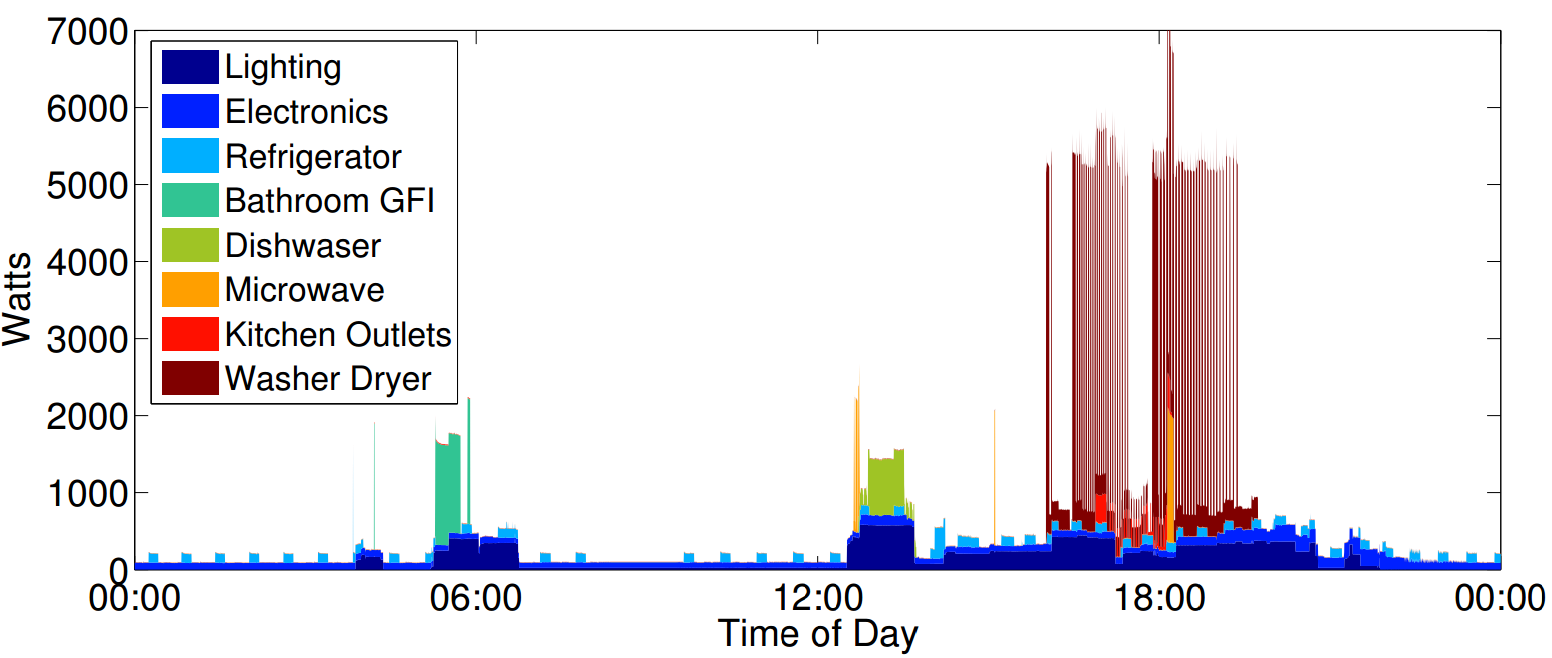
\includegraphics[width=\textwidth]{chapters/introduction-chapters/energy-consumption-house.png}
	\caption{An example of energy consumption of a household over the course of a day \cite{kolter2011redd}.}
	\label{fig:energy-consumption-house}
\end{figure}




If every light in a household would have a unique power draw, that is distinguishable from all other lights, the consumer can get better insight about how lighting is being used in his household. 
With this feedback, a consumer can see which individual lights are being used in the middle of the day for example or in an unoccupied room.
The consumer can then turn the lights off.
Thereby saving energy and monetary costs.



Giving each light a unique signature is an almost intractable problem.
But the advent of smart lights can help with this.
The unique power draw of each light can be managed through VLC (Visible Light Communication).
%With this information that is being sent via VLC, the light can act as a beacon for indoor localization \cite{Kuo:2014:LIP:2639108.2639109}.
%For example a smart-phone could then locate itself inside a building with good accuracy.
%The ID of the LED beacon which is sent via VLC will also propagate via the current that the LED draws.
The information that is transmitted using VLC, will also propagate via the current that the LED draws.
The information that is transmitter must be chosen in such a way that a smart-meter is still able to identify them on a per lamp basis.
And the current that is drawn must have a shape that can be added with similar patterns so that the smart-meter can make sense of this aggregated current and can start to identify if an LED is on or off.






% !TeX root = ../../thesis.tex


\section{Problem Definition}

Energy disaggregation can detect energy consumers based off the distinct power draw that these devices have.
What it cannot yet do, is the disaggregation of appliances that have very similar power draw, such as lighting.


% !TeX root = ../../thesis.tex


\section{Thesis Contributions}

The aim of this thesis is to propose a framework consisting of theoretical methods, hardware and software, so that lights with similar power draw can be distinguished with a single smart-meter.
This thesis takes advantage of advances in two areas: CDMA codes and VLC.

The specific contributions of this thesis are:

\begin{itemize}

	\item Coding methods are analyzed to allow each LED to have a unique power draw. 
	These codes make it possible to identify if an LED is on or off, even when multiple LEDs are modulating and thereby interfering with each others unique current signature.




	\item Hardware is introduced to allow the LEDs to be modulated by a micro controller. 
	This will allow the LEDs propagate their unique signature via either AC or DC. 
	And there is also hardware introduced that can sample the current that all the LEDs are drawing, via either AC or DC.
	The sampled current is then processed by another separate micro controller, which can then state which LEDs are on and which or off.




	\item An evaluation of the proposed hardware and software is carried out, with a testbed which uses standard LED light fixtures. For larger scale evaluations, software simulation is used. 
\end{itemize}


% !TeX root = ../../thesis.tex

\section{Thesis Organization}

The remainder of this thesis is organized as follows.
First the related work and the new proposed method is discussed in \autoref{chp:related-work}.
Then the design requirements are outlined in \autoref{chp:design-requirements}.
In \autoref{chp:cdma} the theory about code sequences is explained.
Next, in \autoref{chp:hardware-design}, the existing hardware and the design of the new hardware is discussed.
In \autoref{chp:evaluation} the hardware and software is evaluated for small scale scenarios and simulations are shown for large scale scenarios.
Finally the work is concluded in \autoref{chp:conclusionsandfuturework} and future work is identified.


% !TeX root = ../../thesis.tex

\chapter{State-of-the-Art}
\label{chp:state-of-the-art}


% what is vlc and how it is used

Visible light communication (VLC) is a short-range optical means of wireless communication using the visible light spectrum.
VLC is made possible by the advances in LED technology.
The interest in VLC has grown since the widespread deployment of LED lighting fixtures for energy efficiency over the normal incandescent light bulb \cite{rajagopal2012ieee}.


Now that VLC allows lighting fixtures to transmit data, research is being done to make indoor localization more precise than with traditional RF-based approaches \cite{Kuo:2014:LIP:2639108.2639109}.
Since the light does not pass through walls and it has less reflection compared to RF, an indoor localization system can be more precise.



Many research papers have successfully recognized home appliances through energy disaggregation with data being collected with a single smart-meter.   
Though they succeed in detecting appliances with unique signatures, lighting is put in a group without mentioning the individual lights \cite{kolter2011redd}.
The reason for this, is because every light has a very similar power draw and therefor a very similar signature and it can not be reliably disaggregated.




% !TeX root = ../../thesis.tex

\chapter{Design Requirements}
\label{chp:design-requirements}

In this chapter, the requirements of both hardware and software will be explained.
First the software side and then the hardware side will be detailed.
Buildings traditionally only have AC power, but there is also research being done \todo{Citation needed, from NL or other origin ???} in using DC power in buildings. 
Therefor each section will also contain the implications on using DC or AC.
In \autoref{fig:overview-diagram} a block diagram can be seen how all components interact with each other.


\begin{figure}[h]
	\centering
	\resizebox {\textwidth} {!} {
		\begin{tikzpicture}

			\node[block] (smart_meter) {Smart-meter};	

			\node[block, left = 1cm of smart_meter] (power) {Power};	
			\draw[line] (power.east) -- (smart_meter.west) node [midway, right] {};		

			% second mod.
			\node[block, right = 4cm of smart_meter] (second_modulator) {Modulator};
			\node[LED, right = 0.5cm of second_modulator] (second_led) {LED};
			\draw[line] (second_modulator.east) -- (second_led.west) node [midway, right] {};

			% first mod.
			\node[block, above = 1cm of second_modulator] (first_modulator) {Modulator};
			\node[LED, right = 0.5cm of first_modulator] (first_led) {LED};
			\draw[line] (first_modulator.east) -- (first_led.west) node [midway, right] {};

			% third mod.
			\node[block, below = 1cm of second_modulator] (third_modulator) {Modulator};
			\node[LED, right = 0.5cm of third_modulator] (third_led) {LED};
			\draw[line] (third_modulator.east) -- (third_led.west) node [midway, right] {};

			\node[dot, right = 2.5cm of smart_meter] (CP) {};

			\draw (smart_meter.east) -- (CP) node [pos=0.3, above] {0222};

			\draw (CP) |- (first_modulator.west) node  [pos=0.75, above] {0011};
			\draw (CP) |- (second_modulator.west) node [pos=0.75, above] {0110};
			\draw (CP) |- (third_modulator.west) node  [pos=0.75, below] {0101};

		\end{tikzpicture}
	}
	\caption{Block diagram how each component interacts with other components.}
	\label{fig:overview-diagram}
\end{figure}


	\section{Encoding}

	To be able to distinguish multiple lights from each other, which are all connected in parallel, each light must have a unique identification sequence of some sort.
	Furthermore, that identification sequence must somehow be detected and interpreted by a smart-meter.


	If the transmission of the identification sequence is done with OOK (on-off keying) in a VLC manner, that encoding will also propagate through the current that is drawn.
	That current flows through the smart meter and then the light source which draws that current can be identified by its unique identification sequence. 


	A problem rises when more than one light source is sending its identification sequence.
	Since the lights are connected in parallel, the current that flows through the smart meter will be the sum of all the currents that are drawn by all the light sources.
	This means that the light sources, which are effectively transmitters, interfere with each other.
	Because of that interference the unique identification sequences which are assigned to each light source, need to be carefully selected.


	The field of telecommunications already faced similar issues: For example multiple cellphones transmitting to the same base station, at the same time, at the same frequency. 
	The solution was to use code sequences that do not posses high cross-correlations, but do have high auto-correlations.
	The specific codes are called Orthogonal codes and Pseudo random noise codes.
	The exact properties, benefits and drawbacks and how they can be used in both DC and AC environments will be discussed in \autoref{chp:cdma}.




	\section{LED Modulator}

	A piece of hardware is needed to modulate a commercial LED.
	This hardware needs to translate the unique identification sequence that is assigned to each light source and modulate the LED.
	The modulation needs to be done in such a way that the aggregated current of all lights can be measured at the smart meter.  
	The hardware should also allow for fast modulating to avoid seeing flickering effects.


	For the design of this hardware, or when using pre-designed hardware, the way the identification sequence translates to the current draw needs to be taken in mind. 
	With AC the applied voltage is a sine wave, which from a positive to a negative voltage.
	So the supplied voltage is never the same and it is zero crossing, meaning that there no current will flow at that point in time.
	And when there is no current flow, there can also be no information encoding.
	This issue must also be taken in mind.



	\section{Smart Meter}

	The smart meter needs to be able to detect relatively small current changes.
	More concretely, it needs to be able to detect the current change when even a single light is modulating, while multiple other lights are on.

	When selecting a method of measuring the current these thing need to be taken into consideration:

	\begin{itemize}
		\item The speed at which the current can be sampled needs to be high enough to be able to correctly sample the current as the LEDs are modulating.

		\item The accuracy of the samples being taken needs to be high enough, so that the modulation of one LED can be detected with consistency.
		In other words, the noise of the samples must be low enough to detect the correct modulation of even one LED.

		\item The applied voltage to the microprocessor cannot be higher than the rated voltage of that microprocessor. This means that the sensitivity (mV / A) of the measuring method needs to be chosen in such a way that the output voltage of the measuring method, is within bounds to not damage the microprocessor.
		The microprocessor cannot handle the negative current, in the case of AC. So an intermediary step needs to take place here to convert it to something the microprocessor can handle, meaning only positive voltages and below the rated voltage of that microprocessor.

	\end{itemize}




















% !TeX root = ../../thesis.tex

\chapter{Code Division Multiple Access}
\label{chp:cdma}

\todo{Should I explain differences TDM/FDM/CDMA ??}

This chapter will explain which CDMA codes are considered and how to measure their performance.
The way in which these codes can be constructed is also explained, as are the environments in which they work well and poorly. 

% !TeX root = ../../thesis.tex

\section{Performance Metrics of a CDMA Sequence}
\label{sec:performance-metrics-cdma}

To be able to objectively determine which code sequence is the best for certain environments, metrics are needed to compare the performance of a sequence.
Such metrics are: auto- and cross-correlation, length of the code and how many unique codes can be produced which are in the same set, meaning with the same length, so that they can be used together in the same system.
Also if the codes can be used in a synchronous only or in an a-synchronous environment has to be considered.


Correlation is a measure for determining how much sequence $X$ is similar to sequence $Y$ and can be found in \autoref{eq:correlation}.
With $L$ being the length of the code and $\tau$ the time-shift.
When sequence $X$ and $Y$ are the same sequence, we speak of the autocorrelation.
When they are two different sequences, we speak of the cross-correlation. 

\begin{equation}
	R(\tau)_{xy} = \displaystyle\sum_{i = 0} ^ {L - 1} x(i) \times y(i + \tau) {\text{  with $\tau = 0, 1, 2, \dotsc, L$}}
	\label{eq:correlation}
\end{equation}


%commented out because this will never be used and therefor only adds unnecessary text

%Another way to calculate the correlation between two sequences is to count the number of agreements and disagreements between the two sequences, see \autoref{eq:correlation-a-d}, this comes in handy when comparing two digital sequences, which both have $0$ and $1$ signal levels.

%\begin{equation}
%	R(\tau) = \text{\# of agreements} - \text{\# of disagreements} 
%	\label{eq:correlation-a-d}
%\end{equation}




The properties of an ideal set of codes should be, that the autocorrelation for each code in the set should be $0$ for each time-shift $\tau \neq 0$, at $\tau = 0$ the autocorrelation should be $L$, this value would than be a peak value for which we can identify if this code is present in the received signal.
If the signal is the sampled current and the code is the ID of a LED, then we can say the LED is on when the auto-correlation peak is seen.
The ideal cross-correlation properties should be $0$ for every time-shift $\tau$, so that no code interferes with any other code, hereby causing no MAI (Multiple Access Interference).



The length of a code is also of importance, because each chip of the code has to be transmitted.
Assuming a constant modulating frequency, the time it takes to transmit a code sequence is proportional to the length of that code sequence.
The length of the code will also determine, to some extent, the number of codes in the same set.
The number of codes in the same set determines the scalability of the system.






% !TeX root = ../../thesis.tex

\section{Orthogonal Sequences}
\label{sec:orthogonal-sequences}

Orthogonal sequences, also known as Walsh-Hadamard sequences, are sequences which are created using a Hadamard matrix.
Hadamard matrices are square $n \times n$ matrices which are recursively generated.
Starting with a $1 \times 1$ matrix: 
		$H_{1} = \begin{bmatrix} 1 \end{bmatrix}$, then 
		$H_{2} = \begin{bmatrix} 1 & 1 \\ 1 & -1 \end{bmatrix}$.
See \autoref{eq:hadamard-matrix-creation} for a general recursive formula to generate other ranks of Hadamard matrices \cite{714616}.

\begin{equation}
	H_{2n} = 
	\begin{bmatrix} 
		H_n & H_n \\ 
		H_n & -H_n 
	\end{bmatrix}
	\label{eq:hadamard-matrix-creation}
\end{equation}

The matrix can also be filled with binary values: $0$ and $1$. In that case the general recursive formula is stated in \autoref{eq:hadamard-matrix-creation-bin}. 

\begin{equation}
	H_{2n} = 
	\begin{bmatrix} 
		H_n & H_n \\ 
		H_n & \overline{H_n}
	\end{bmatrix}
	\label{eq:hadamard-matrix-creation-bin}
\end{equation}




The Hadamard matrix has the property that every row in the matrix, apart from the first row, is orthogonal to every other row.
And apart from the first row, all other rows have the exact same number of $+1$s and $-1$s, meaning the sum of an entire row is equal to zero.

Hadamard matrices exist for every power of $2$, so the code length is also a power of $2$.
For $\tau = 0$, the cross-correlation is $0$, but when $\tau \neq 0$ not all the rows are orthogonal anymore.
\cite{1182447} proved that an Hadamard matrix of size $2^P$ could be divided into $P + 1$ subsets of rows, where one row could be selected giving $P + 1$ orthogonal rows for each time-shift $\tau$.
These codes are called Cyclically Orthogonal Walsh Hadamard Codes (COWHC).

All rows of the matrix have the property that the autocorrelation at $\tau = 0$ is equal to $L$.
But when $\tau \neq 0$, undesirable behavior occurs as can be seen in \autoref{fig:autocorr-hadamard}.
The autocorrelation function has several high peaks where only one is desired.
This means that if a transmitter sends an encoded message with this code and the receiver does not know when in time the start of the message is, the receiver would get false positives for data.

\begin{figure}[t]
	\centering
	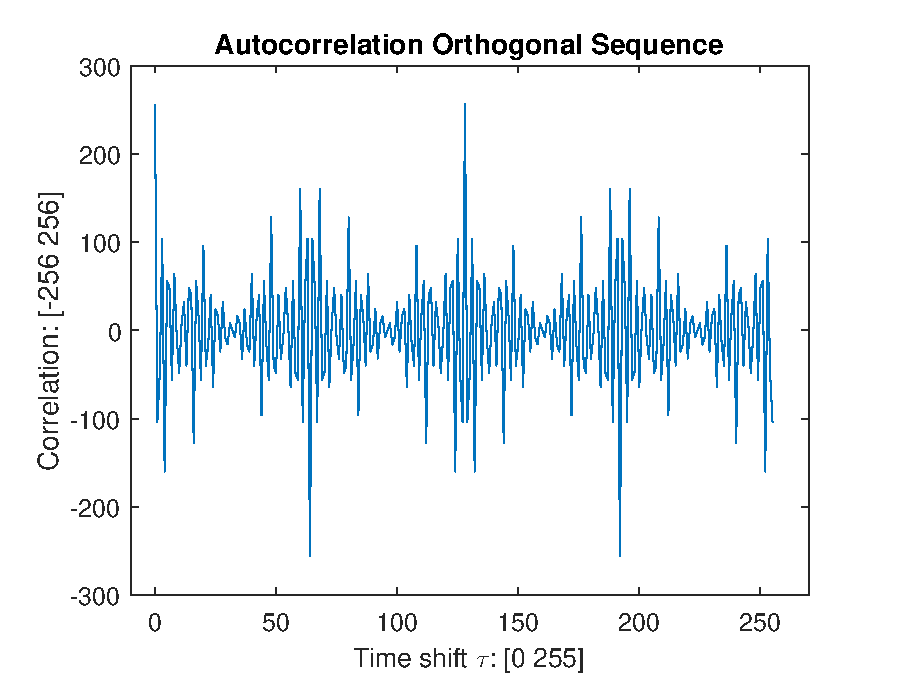
\includegraphics[width=\textwidth]{chapters/cdma-chapters/autocorr-hadamard.eps}
	\caption{Autocorrelation of orthogonal sequence with row index 120 of length 256.}
	\label{fig:autocorr-hadamard}
\end{figure}


Only a small subset of the codes (COWHC) have $0$ cross-correlation for every time-shift $\tau$, with code length $L$ there are $\log_2 L$ codes in the set, which makes these codes not scalable. Also the autocorrelation does not have a clear peak to identify the code.

The entire set of orthogonal codes of length $L$, has $L - 1$ codes in the set which does make it a scalable set.
But the auto- and crosscorrelation only have the desired properties when the codes are sent synchronously. 
\todo{Extra conclusion like: the transmitters/LEDs cannot be synchronized, or does that come later...}

% !TeX root = ../../thesis.tex

\section{Pseudorandom Noise Sequences}
\label{sec:pn-sequences}

PN sequences are sequences which look like they are randomly generated but they are easily generated in software or hardware.
They are generated with linear shift registers of length $n$.
The sequences have the following noise-like properties~\cite{mitra2008pseudo}:

\begin{itemize}
	\item Balance property:	Any PN sequence of length $L = 2^n - 1$ contains exactly $2^{n-1}$ ones and exactly $2^{n-1} - 1$ zeros.

	\item Runs property: A run is a subset of the sequence where all the consecutive numbers are the same. In any PN sequence, $1/2$ of the runs have length 1, $1/4$ have length 2, $1/8$ have length 3 and so on.

	\item Autocorrelation property: The autocorrelation function of a PN sequence will take on two values as can be seen in \autoref{eq:autocorr-pn} and \autoref{fig:autocorr-pn}.


\end{itemize}

\begin{equation}
	\label{eq:autocorr-pn}
	R(\tau) = 
		\begin{cases}
			L    & \quad \text{if } \tau = 0 \\
			-1   & \quad \text{if } \tau \neq 0 \\
		\end{cases}
\end{equation}

\begin{figure}[h]
	\centering
	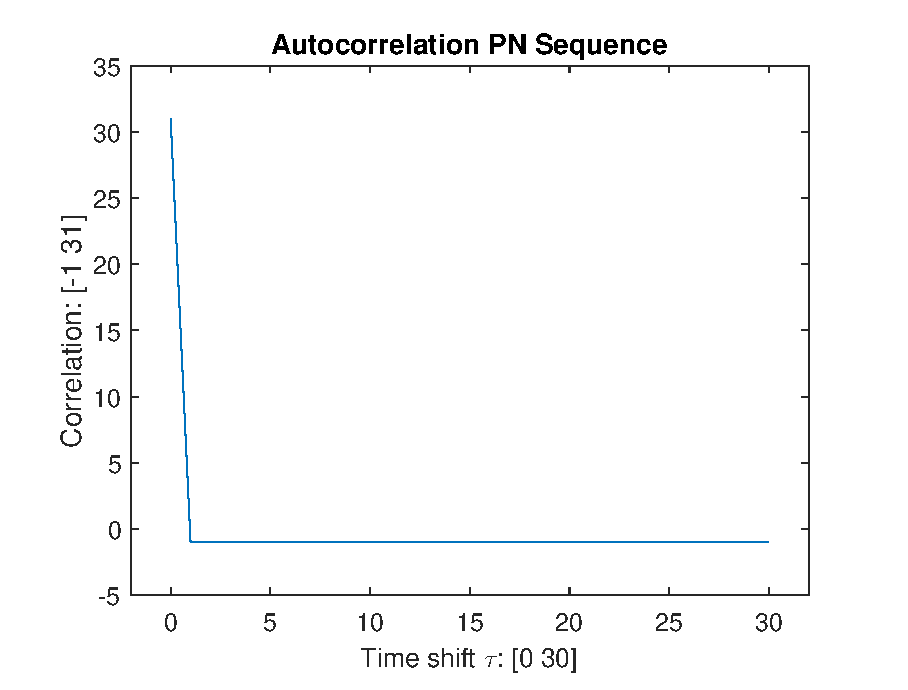
\includegraphics[width=\textwidth]{chapters/cdma-chapters/autocorr-pn.eps}
	\caption{Autocorrelation of PN sequence of length 31.}
	\label{fig:autocorr-pn}
\end{figure}

PN sequences are generated using a linear feedback shift register (LFSR) \cite{Wang:1988:LFS:52007.52024}.
\autoref{fig:lfsr} shows an $n$ length LFSR with some XOR gates attached to it.
The LFSR is defined entirely by the feedback function, also called a characteristic polynomial.
It determines the length and the type of sequence generated.
The polynomial looks like \autoref{eq:lfsr-polynomial}.

\begin{equation}
	\label{eq:lfsr-polynomial}
	p(x) = x^n + C_{n-1} x^{n-1}  + C_{n-2} x^{n-2} + \dotsc + C_{2} x^{2}  + C_{1} x  + C_{0}
\end{equation}

\begin{figure}[h]
	\centering
	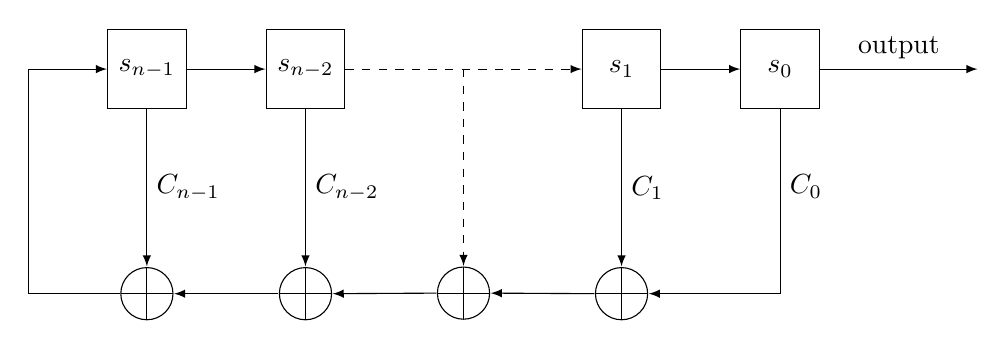
\begin{tikzpicture}


		\node[block                  ] (last_register) {$s_{n-1}$};
		\node[block, right = 1cm of last_register] (second_last_register) {$s_{n-2}$};
		\draw[line] (last_register.east) -- (second_last_register.west) ;

		\node[block, right = 3cm of second_last_register] (second_register) {$s_{1}$};
		\node[block, right = 1cm of second_register] (mid_register) {$s_{0}$};
		\draw[line] (second_register.east) -- (mid_register.west) ;

		\draw[dashed, line] (second_last_register.east) -- (second_register.west) ;

		\node[coordinate, right = 2cm of mid_register] (output_point) {};
		\draw[line] (mid_register.east) -- (output_point.west) node [midway, above] {output};

		\node[XOR, scale=2, below = 2cm of second_register] (first_xor) {};
		\draw[line] (second_register.south) -- (first_xor.north) node [midway, right] {$C_1$};
		\draw[line] (mid_register.south) |- (first_xor.east) node [pos=0.21, right] {$C_0$};

		\node[coordinate, right = 1.5cm of second_last_register] (h) {};
		\node[XOR, scale=2, below = 2.5cm of h] (mid_xor) {};
		\draw[line] (first_xor.west) -- (mid_xor.east) ;
		\draw[dashed, line] (h.south) -- (mid_xor.north) ;

		\node[XOR, scale=2, below = 2cm of second_last_register] (second_last_xor) {};
		\node[XOR, scale=2, below = 2cm of last_register] (last_xor) {};

		\draw[line] (second_last_register.south) -- (second_last_xor.north) node [midway, right] {$C_{n-2}$};
		\draw[line] (mid_xor.west) -- (second_last_xor.east) ;
		
		\draw[line] (second_last_xor.west) -- (last_xor.east) ;
		\draw[line] (last_register.south) -- (last_xor.north) node [midway, right] {$C_{n-1}$};

		\node[coordinate, left = 1cm of last_register] (return_point) {};
		
		\draw[line] (last_xor.west) -| (return_point) -- (last_register.west) ;




	\end{tikzpicture}
	\caption{Linear feedback shifter register of length $n$, with XOR gates.}
	\label{fig:lfsr}
\end{figure}


For PN sequences, there exists no formula for the cross-correlation of two different PN sequences. 
Exhaustive analysis is required to find out which sequences or entire sets have the cross-correlation characteristics that are good enough for the user's application.

The size of the code set is limited.
For a LFSR with $n$ registers, the maximum number of possible codes $C$ is given by \autoref{eq:num-of-pn-codes} \cite{mutagi1996pseudo}, where $P_i$ are the prime factors of $2^n - 1$ and $\alpha_i$ is the power of $i$th prime factor.

\begin{equation}
	\label{eq:num-of-pn-codes}
	C = \frac{1}{n} \prod \{ P_{i} ^ {(\alpha_i - 1)} \times (P_i - 1) \}
\end{equation}

For example when using a LFSR of size $n = 6$, $2^n - 1 = 63$, which can be factored into $3^2 \times 7$.
Giving $P_1 = 3$, $P_2 = 7$, $\alpha_1 = 2$ and $\alpha_2 = 1$.
Thus, the maximum number of codes is: $C = \frac{1}{6} \times \{ 3^{2 - 1} \times (3 - 1) \} \times \{ 7^{1 - 1} \times (7 - 1) \} = 6$.
Another example: Say there are going to be 144 user, so 144 codes are needed. 
This means a code length of 4095 chips.
















\subsection{Gold Sequences}
\label{subsec:gold-sequences}

Gold sequences are a type of PN sequence. 
They are created by using two LFS registers as shown in \autoref{fig:gold-lfsr}.
In this figure there are two vectors $s$ and $t$ and two polynomials $C$ and $D$.
For a sequence to be constructed in this way that is a Gold sequence, only preferred pairs of polynomials can be used \cite{kedia2012comparative}.
When we have the polynomials $p(x)$ and $q(x)$, which are a preferred pair and produces the PN sequences $d_1$ and $d_2$ respectively, the resulting set of Gold codes is defined as can be seen in \autoref{eq:gold-def}, where $T^n$ represent the cyclic shift of $n$ bits.

\begin{equation}
	\label{eq:gold-def}
	Gold(d_1, d_2) = \{ d_1, d_2, d_1 \oplus d_2, d_1 \oplus Td_2, d_1 \oplus T^2d_2, \dotsc, d_1 \oplus T^{L - 1}d_2 \}
\end{equation}


\begin{figure}[h]
	\centering
	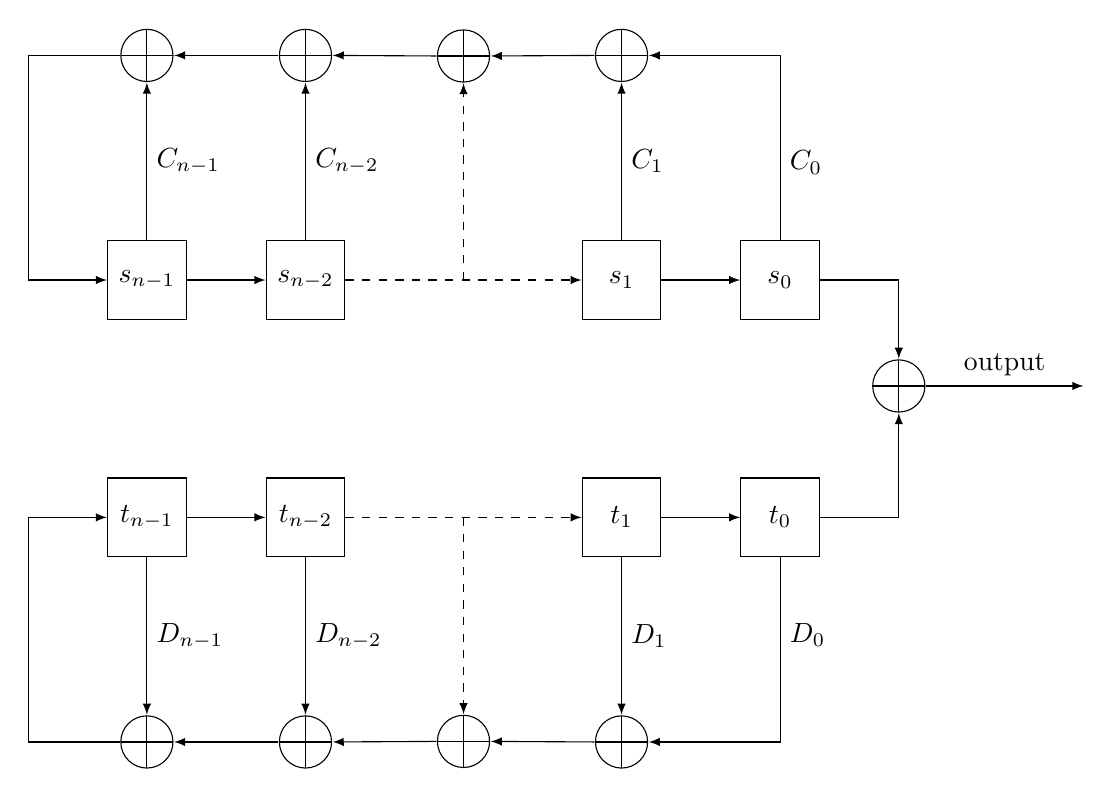
\begin{tikzpicture}

		\node[block                  ] (last_register1) {$s_{n-1}$};
		\node[block, right = 1cm of last_register1] (second_last_register1) {$s_{n-2}$};
		\draw[line] (last_register1.east) -- (second_last_register1.west) ;

		\node[block, right = 3cm of second_last_register1] (second_register1) {$s_{1}$};
		\node[block, right = 1cm of second_register1] (mid_register1) {$s_{0}$};
		\draw[line] (second_register1.east) -- (mid_register1.west) ;

		\draw[dashed, line] (second_last_register1.east) -- (second_register1.west) ;

		\node[coordinate, right = 1cm of mid_register1] (output_point1) {};

		\node[XOR, scale=2, above = 2cm of second_register1] (first_xor1) {};
		\draw[line] (second_register1.north) -- (first_xor1.south) node [midway, right] {$C_1$};
		\draw[line] (mid_register1.north) |- (first_xor1.east) node [pos=0.21, right] {$C_0$};

		\node[coordinate, right = 1.5cm of second_last_register1] (h1) {};
		\node[XOR, scale=2, above = 2.5cm of h1] (mid_xor1) {};
		\draw[line] (first_xor1.west) -- (mid_xor1.east) ;
		\draw[dashed, line] (h1.north) -- (mid_xor1.south) ;

		\node[XOR, scale=2, above = 2cm of second_last_register1] (second_last_xor1) {};
		\node[XOR, scale=2, above = 2cm of last_register1] (last_xor1) {};

		\draw[line] (second_last_register1.north) -- (second_last_xor1.south) node [midway, right] {$C_{n-2}$};
		\draw[line] (mid_xor1.west) -- (second_last_xor1.east) ;
		
		\draw[line] (second_last_xor1.west) -- (last_xor1.east) ;
		\draw[line] (last_register1.north) -- (last_xor1.south) node [midway, right] {$C_{n-1}$};

		\node[coordinate, left = 1cm of last_register1] (return_point1) {};
		
		\draw[line] (last_xor1.west) -| (return_point1) -- (last_register1.west) ;

		%%%%%%%%%%%%%%%%%%%%%%%%%%%%%%%%%%%%%%%%%%%%%%%%%%%%%%%%%%%%%%%%%%%%%%%%%%%%


		\node[block, below = 2cm of last_register1] (last_register) {$t_{n-1}$};
		\node[block, right = 1cm of last_register] (second_last_register) {$t_{n-2}$};
		\draw[line] (last_register.east) -- (second_last_register.west) ;

		\node[block, right = 3cm of second_last_register] (second_register) {$t_{1}$};
		\node[block, right = 1cm of second_register] (mid_register) {$t_{0}$};
		\draw[line] (second_register.east) -- (mid_register.west) ;

		\draw[dashed, line] (second_last_register.east) -- (second_register.west) ;

		\node[coordinate, right = 1cm of mid_register] (output_point) {};

		\node[XOR, scale=2, below = 2cm of second_register] (first_xor) {};
		\draw[line] (second_register.south) -- (first_xor.north) node [midway, right] {$D_1$};
		\draw[line] (mid_register.south) |- (first_xor.east) node [pos=0.21, right] {$D_0$};

		\node[coordinate, right = 1.5cm of second_last_register] (h) {};
		\node[XOR, scale=2, below = 2.5cm of h] (mid_xor) {};
		\draw[line] (first_xor.west) -- (mid_xor.east) ;
		\draw[dashed, line] (h.south) -- (mid_xor.north) ;

		\node[XOR, scale=2, below = 2cm of second_last_register] (second_last_xor) {};
		\node[XOR, scale=2, below = 2cm of last_register] (last_xor) {};

		\draw[line] (second_last_register.south) -- (second_last_xor.north) node [midway, right] {$D_{n-2}$};
		\draw[line] (mid_xor.west) -- (second_last_xor.east) ;
		
		\draw[line] (second_last_xor.west) -- (last_xor.east) ;
		\draw[line] (last_register.south) -- (last_xor.north) node [midway, right] {$D_{n-1}$};

		\node[coordinate, left = 1cm of last_register] (return_point) {};
		
		\draw[line] (last_xor.west) -| (return_point) -- (last_register.west) ;

		%%%%%%%%%%%%%%%%%%%%%%%%%%%%%%%%%%%%%%%%%%%%%%%%%%%%%%%%%%%%%%%%

		\node[XOR, scale=2, below = 1cm of output_point1] (gold_xor) {};
		\draw[line] (mid_register1) -| (gold_xor) ;
		\draw[line] (mid_register) -| (gold_xor) ;
		\node[coordinate, right = 2cm of gold_xor] (gold_output) {} ;
		\draw[line] (gold_xor.east) -- (gold_output.west) node [midway, above] {output};


	\end{tikzpicture}
	\caption{Two linear feedback shifter registers of length $n$, with XOR gates to produce a set of Gold sequences.}
	\label{fig:gold-lfsr}
\end{figure}

\begin{figure}
	\centering
	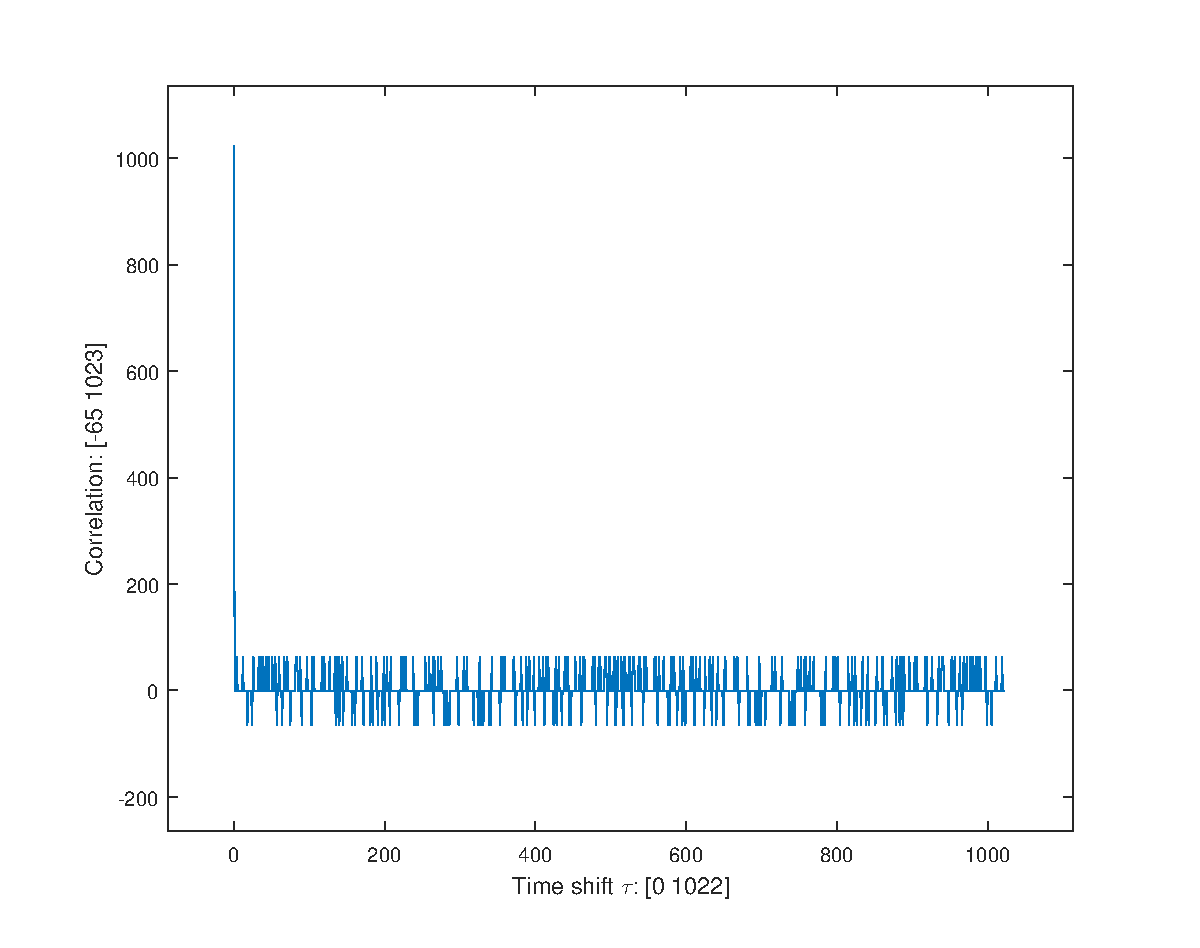
\includegraphics[width=\textwidth]{chapters/cdma-chapters/autocorr-gold.eps}
	\caption{Autocorrelation of one Gold sequence of length 1023.}
	\label{fig:autocorr-gold}
\end{figure}


\begin{figure}
	\centering
	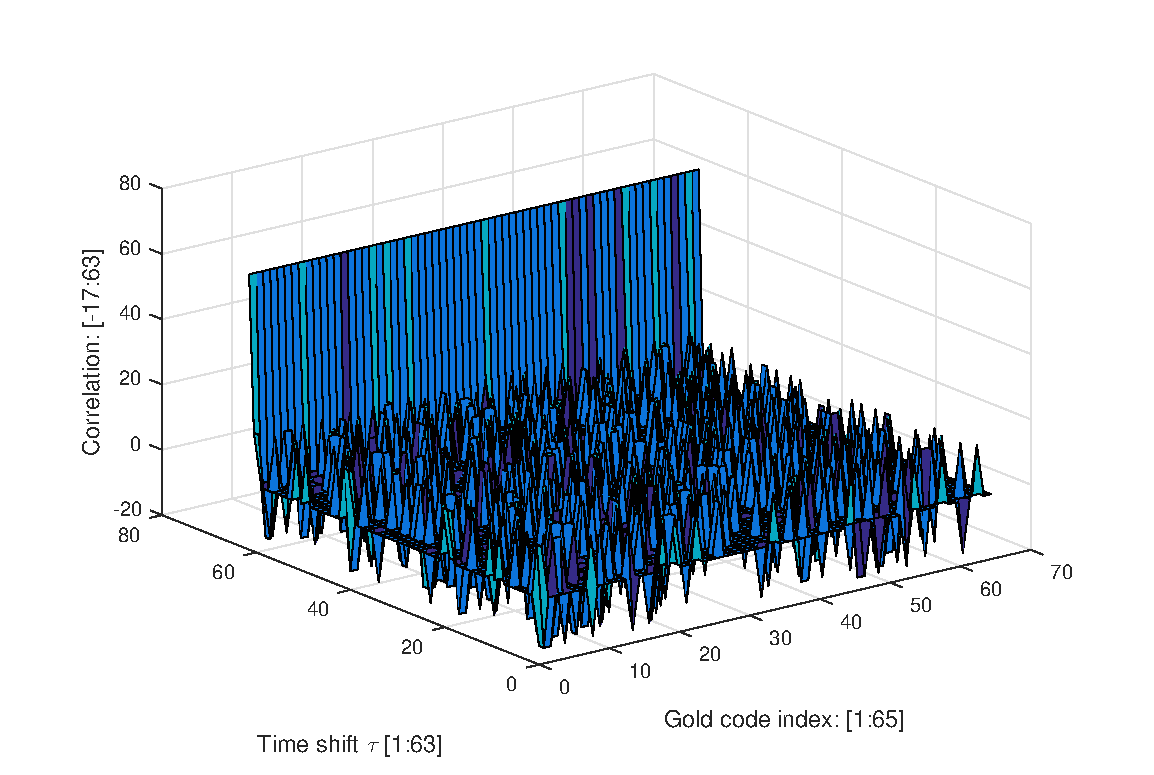
\includegraphics[width=\textwidth]{chapters/cdma-chapters/autocorr-gold-3d.eps}
	\caption{Autocorrelation of all Gold codes in the same set of length 63.}
	\label{fig:autocorr-gold-3d}
\end{figure}




The autocorrelation properties of Gold sequences are not as good as that of the PN sequences, as can be seen from \autoref{fig:autocorr-gold-3d}.
Apart from the original two PN sequences the autocorrelation values are not two-valued, but are four-valued.
See \autoref{eq:autocorr-gold} and \autoref{eq:gold-t(n)} for the autocorrelation properties of Gold sequences.

\begin{equation}
	\label{eq:autocorr-gold}
	R(\tau) = 
		\begin{cases}
			L    							& \quad \text{if } \tau = 0 \\
			\{ -t(n), \ -1, \ t(n) - 2  \} 	& \quad \text{if } \tau \neq 0 \\
		\end{cases}
\end{equation}

\begin{equation}
	\label{eq:gold-t(n)}
	t(n) = 
		\begin{cases}
			1 + 2^{\frac{n+1}{2}} & \quad \text{for odd } n \\
			1 + 2^{\frac{n+2}{2}} & \quad \text{for even } n \\
		\end{cases}
\end{equation}

See \autoref{eq:corsscorr-gold} and \autoref{eq:gold-t(n)} for the cross-correlation properties of Gold sequences \cite{mitra2008pseudo}.

\begin{equation}
	\label{eq:corsscorr-gold}
	R_{xy}(\tau) = 	\{ -t(n), -1, t(n) - 2  \} 
\end{equation}


From these equations it is clear to see that the absolute maximum cross-correlation is bounded by $t(n)$.

When $n$ is chosen to be odd, something can be said about the approximate frequency of occurrence of the cross-correlation values, see \autoref{tbl:freq-occurence-gold-cross-correlation} \cite{holmes2007spread}.

\begin{table}[h]
	\centering
	\begin{tabular}{ | l | l | }

		\hline
		$R_{xy}(\tau)$ 	& Frequency of occurrence	\\ \hline

		$-1$			& 0.5					 	\\ \hline
		$-t(n)$			& 0.25						\\ \hline
		$t(n) - 2$		& 0.25						\\ \hline

		

	\end{tabular}
	\caption{Table containing the approximate frequency of occurrence for all the cross-correlation values for $n$ odd.}
	\label{tbl:freq-occurence-gold-cross-correlation}
\end{table}

The Gold sequences are not all balanced like the PN sequences. 
Roughly half of the sequences in the same set are balanced, sometimes this can be as high as three quarters. \cite{holmes2007spread}


The Gold sequences posses good auto- and crosscorrelation, suitable for a-synchronous usage.
\todo{Also state that this is extra good, because the LEDs/transmitters cannot be synchronized ???}
Also the codes scale well.
With a LFSR of length $n$, the sequence length is $L = 2^n - 1$ and the number of sequences is $C = 2^n + 1$.

\todo{What information is really needed and which (like this table) is not necessary}












% !TeX root = ../../thesis.tex

\section{Mapping Problem}
\label{sec:mapping-problem}

The coding methods as discussed in \autoref{subsec:orthogonal-sequences} and \autoref{subsec:pn-sequences} are used in the field of telecommunication.
Since these signals are analog radio waves, the symbols are $+1$ and $-1$ and they are balanced around $0$.
The LFS registers used with the generation of PN and gold sequences, only output zeros and ones.
For the use with radio-signals a code sequence is mapped to a form with $+1$ and $-1$, where the original $0$ is mapped to $+1$ and the original $1$ is mapped to $-1$ \cite{cdma-mapping-symbols-ref}.



First the equations are shown, how to calculate the correlation for a particular code when the code sequences from all the transmitters only have $+1$ and $-1$ symbols. 
In \autoref{eq:eqns-correlation-normal-symbols} it is shown how to calculate the correlation $R$, where we use \autoref{eq:correlation} and where $s(t)$ is the received signal which is the composed signal of $m$ distinct codes, which all use the $+1$ and $-1$ symbols and where $c^r_1(t)$ is the code sequence, with symbols $+1$ and $-1$, for which we want to calculate the correlation.


\begin{equation}
	\begin{array}{l}
		R_{sc^r_{1}} = \displaystyle\sum_{t = 0} ^ {L - 1} s(t) \times c^r_1(t)	 \\
		s(t) = \displaystyle\sum_{i = 1} ^ {m} c^r_i(t) \\
		R_{sc^r_{1}} = \displaystyle\sum_{t = 0} ^ {L - 1} \Bigg\{ c^r_1(t) \times  \displaystyle\sum_{i = 1} ^ {m} c^r_i(t) \Bigg\} 
	\end{array} 
	\label{eq:eqns-correlation-normal-symbols}
\end{equation}


%The following proof \todo{Are we calling this a proof ??} shows how to calculate the correlation when the coding sequence consists of $+1$ and $-1$ symbols: 

%\begin{proof}
%	Let $s(t)$ be the received signal which is the composed signal of $m$ distinct codes.\\
%	And let $c_i(t)$ be the code sequence $i$, and let $c_1(t)$ be the code for which we want to check if there is information there. \\
%
%	\begin{align*}
%		R(\tau)_{xy} = \displaystyle\sum_{t = 0} ^ {L - 1} x(t) \times y(t + \tau)	\tag{See \autoref{eq:correlation}}
%		\\ \tau = 0,\ x = s(t),\ y = c_1(t)	
%		\\ R(0)_{sc_{1}} = \displaystyle\sum_{t = 0} ^ {L - 1} s(t) \times c_1(t)
%		\\ s(t) = \displaystyle\sum_{i = 1} ^ {m} c_i(t)														
%		\\ R(0)_{sc_{1}} = \displaystyle\sum_{t = 0} ^ {L - 1}  \Bigg\{  c_1(t)	\times \displaystyle\sum_{i = 1} ^ {m} c_i(t) \Bigg\}
%		\\ R(0)_{sc_{1}} = \displaystyle\sum_{t = 0} ^ {L - 1} \Bigg\{ c_1(t) \times c_1(t) + c_1(t) \times  \displaystyle\sum_{i = 2} ^ {m} c_i(t) \Bigg\} 
%		\\ R(0)_{sc_{1}} = \displaystyle\sum_{t = 0} ^ {L - 1} c_1(t) \times c_1(t) + \displaystyle\sum_{t = 0} ^ {L - 1} \Bigg\{ c_1(t) \times  \displaystyle\sum_{i = 2} ^ {m} c_i(t) \Bigg\} 
%		\\ R(0)_{sc_{1}} = L + \displaystyle\sum_{t = 0} ^ {L - 1} \Bigg\{ c_1(t) \times  \displaystyle\sum_{i = 2} ^ {m} c_i(t) \Bigg\} 
%	\end{align*}

%\end{proof}

The correlation calculation holds for any sequence with $+1$ and $-1$ symbols.
For example: Assume $c^r_1 = \{ -1, 1, -1, -1, -1 \}$ and $c^r_2 = \{ 1, -1, -1, 1, -1 \}$.
Note that code $c^r_1$ is not balanced, the sum is equal to $-3$, code $c^r_2$ is balanced because the sum is equal to $-1$.
Also note that these sequences are completely chosen at random, the codes are not orthogonal, pn or gold sequences.
These codes are the IDs of transmitters 1 and 2, respectively.
Also assume that these codes are transmitted at the same time to create $s = c^r_1 + c^r_2 = \{ 0, 0, -2, 0, -2 \}$.
The calculated correlation using \autoref{eq:eqns-correlation-normal-symbols} will now be: $R_{sc^r_{1}} = 4$ and $R_{sc^r_{2}} = 4$.
These are the correlation results when codes are used with $+1$ and $-1$ symbols.
%This example will be used again later in this section to compare when different symbols are used.

The result of \autoref{eq:eqns-correlation-normal-symbols} is the sum of all the correlations. 
If the code that is being correlated with, is present in the signal $s(t)$ then one of the outcomes of the correlation will be the peak auto-correlation $L$ then we can write the total correlation as follows: $R_{sc_{1}} = L + \displaystyle\sum_{t = 0} ^ {L - 1} \Bigg\{ c_1(t) \times  \displaystyle\sum_{i = 2} ^ {m} c_i(t) \Bigg\} $, where the result is the auto-correlation $L$ plus all the other correlations.
If the orthogonal sequences were used all the other correlations are zero.
If the Gold sequences were used each of the other correlations could be one of the values as stated in \autoref{eq:corsscorr-gold}.
This is where the multiple access interference shows.







The above correlation calculation only holds, when using a coding sequence which has $+1$ and $-1$ symbols.
However, for the states of the LEDs we can only choose between an on or off state with OOK, so a $1$ or a $0$.
This means a different correlation calculation is required.
First a formula for the mapping from $+1$ to zero and $-1$ to one is needed.
The formula can be found in \autoref{eq:radio-to-bin}, where $r$ denotes the $+1$ or $-1$ symbols and the outcome $b$ will be our binary value, $0$ or $1$.
This mapping formula is based on the mapping used by PN sequences to work with wireless communication
A PN sequence outputs zeros and ones and these are mapped to $+1$ and $-1$ respectively \cite{cdma-mapping-symbols-ref}.
 
\begin{equation}
	b = \frac{1 - r}{2}
	\label{eq:radio-to-bin}
\end{equation}


The codes that were used in the example above, can now be mapped to $0$ and $1$ symbols.
This results in the following codes: $c^b_1 = \{ 1, 0, 1, 1, 1 \}$ and $c^b_2 = \{ 0, 1, 1, 0, 1 \}$.
The $b$ notation indicates that these sequences consists of $0$ and $1$ symbols.



The previous equation (\autoref{eq:eqns-correlation-normal-symbols}) can now be altered to incorporate the fact that the LEDs work with a one and zero state.
In \autoref{eq:eqns-correlation-binary-symbols} it is shown how the correlation formula changes when the codes that are used for the LEDs now have $0$ and $1$ values instead of the $+1$ and $-1$ values.
In \autoref{eq:eqns-correlation-binary-symbols} the new correlation $\hat{R}$ is calculated, where $c^r_i(t)$ is the code sequence $i$ and consists of symbols $-1$ and $+1$, and $c^b_j(t)$ is the code sequence $j$ and consists of symbols $1$ and $0$ and where $s(t)$ is the received signal which is the composed signal of $m$ distinct codes.
To clarify: The codes that the LEDs use have values $0$ and $1$ due to the OOK, the code that is being correlated with at the receiver or current-sampler side still uses the $+1$ and $-1$ symbols.








The altered correlation calculation, denoted by $\hat{R}$ shows different results than the previous result $R$.
Where $R_{sc_{1}} = \displaystyle\sum_{t = 0} ^ {L - 1} \Bigg\{ c^r_1(t) \times  \displaystyle\sum_{i = 1} ^ {m} c^r_i(t) \Bigg\} $ and $\hat{R}_{sc^r_{1}} = \frac{m}{2} \times \displaystyle\sum_{t = 0} ^ {L - 1} c^r_1(t) - \frac{1}{2} \times \displaystyle\sum_{t = 0} ^ {L - 1}  \Bigg\{ c^r_1(t) \times \displaystyle\sum_{i = 1} ^ {m} c^r_i(t) \Bigg\}$.
We can write it such that $R$ will become a function of $\hat{R}$ as can be seen in \autoref{eq:final-mapped-correlation-function}.
With this equation we get the same output domain as with the normal correlation formula used for the codes that have $+1$ and $-1$ symbols.

\begin{equation}
	\begin{array}{l}
		\hat{R}_{sc^r_{1}} = \displaystyle\sum_{t = 0} ^ {L - 1} s(t) \times c^r_1(t)	 \\
		s(t) = \displaystyle\sum_{i = 1} ^ {m} c^b_i(t) = \displaystyle\sum_{i = 1} ^ {m} \frac{1 - c^r_i(t)}{2} \\
		\hat{R}_{sc^r_{1}} = \displaystyle\sum_{t = 0} ^ {L - 1} \Bigg\{  c^r_1(t)	\times \displaystyle\sum_{i = 1} ^ {m} \frac{1 - c^r_i(t)}{2}  	\Bigg\} \\
		\hat{R}_{sc^r_{1}} = \frac{m}{2} \times \displaystyle\sum_{t = 0} ^ {L - 1} c^r_1(t) - \frac{1}{2} \times \displaystyle\sum_{t = 0} ^ {L - 1}  \Bigg\{ c^r_1(t) \times \displaystyle\sum_{i = 1} ^ {m} c^r_i(t) \Bigg\}
	\end{array} 
	\label{eq:eqns-correlation-binary-symbols}
\end{equation}



\begin{equation}
	R_{sc^r_{1}} = m \times \displaystyle\sum_{t = 0} ^ {L - 1} c^r_1(t) - 2 \times \hat{R}_{sc^r_1}
	\label{eq:final-mapped-correlation-function}
\end{equation}


When the transmitters or LEDs in this case, transmit the codes $c^b_1$ and $c^b_2$, the following signal $s$ would be created: $s = c^b_1 + c^b_2= \{ 1, 1, 2, 1, 2 \}$.
\autoref{eq:eqns-correlation-binary-symbols} can now be used to calculate the new correlation $\hat{R}$: $\hat{R}_{sc^r_{1}} = -5$ and $\hat{R}_{sc^r_{2}} = -3$.
These results are not the same as with the previous correlation results, where the results were 4 and 4, respectively.
This is because $R$ and $\hat{R}$ cannot be compared, instead the results obtained from $\hat{R}$ need to be mapped to $R$.
The values obtained using $\hat{R}$ can now be mapped to $R$ by using \autoref{eq:final-mapped-correlation-function}. %($\hat{R}_{sc^r_{1}} = -5$ and $\hat{R}_{sc^r_{2}} = -3$)
For this equation we also need the sum of the code sequences, which were already calculated in the beginning of the example to show that one of the code sequences is not balanced.
The sums are: $\displaystyle\sum c^r_1 = -3$ and $\displaystyle\sum c^r_2 = -1$.
To obtain $R$: $R_{sc^r_{1}} = m \times \displaystyle\sum c^r_1 - 2 \times \hat{R}_{sc^r_1}  = 2 \times -3 - 2 \times -5 = 4$ and $R_{sc^r_{2}} = m \times \displaystyle\sum c^r_2 - 2 \times \hat{R}_{sc^r_2} = 2 \times -1 -2 \times -3 = 4$.
And these correlation results are the same as the correlation results as with the codes which had $-1$ and $+1$ symbols.
Hence, we show that any sequence can be mapped from $-1$ and $+1$ symbols to $0$ and $1$ symbols and still get correct correlation results.




In \autoref{eq:final-mapped-correlation-function} the sum of the sequence used to correlate with, is needed. 
The sum of the sequence depends on the sequence used, when using orthogonal codes the sum will be zero, see \autoref{subsec:orthogonal-sequences}.
If the sum is equal to zero, the factor $m$ will not matter.
However when the sequence used is a PN sequence or a balanced Gold sequence, the sum will be $-1$.
The sum will be $-1$ due to the fact of the balance property of the PN sequences, as explained in \autoref{subsec:pn-sequences}.
The sequence will have exactly $2^{n-1}$ ones, where the ones will be mapped to $-1$ and the sequence will have exactly $2^{n-1} -1$ zeros, which will be mapped to $1$.
These mappings can be found when inversing \autoref{eq:radio-to-bin}, this yields: $r = 1 - 2 \times b$.
When we calculate the sum of the sequence we get: $2^{n-1} \times -1 + (2^{n-1} - 1) \times 1 = -1$.
Because the sum is equal to $-1$: $R = -m - 2 \times \hat{R}$, and then $m$, the number of signals, is important.
When using an unbalanced Gold sequence, the sum of that sequence is not equal to $-1$.
All the chips of the unbalanced Gold sequence can be added, in order to find the sum of this particular sequence and use the outcome to calculate the correct correlation value as we have done for the example with code $c^r_1$.











% !TeX root = ../../thesis.tex

\section{Interference Solution}
\label{sec:interference-solution}

In the previous sections, interference was discussed when using a CDMA approach.
When there are too many transmitters on the same channel, at the same time, the interference can be so great that it destroys a code sequence of one or more transmitters.
This is not a problem for Orthogonal sequences, since they have no cross correlation, when transmitted synchronously (See \autoref{sec:orthogonal-sequences}).
But this is an issue for Gold sequences. \todo{Should also mention PN sequences in general, and then the table with the calculated cross correlation per length ????}
As stated in \autoref{subsec:gold-sequences}, the cross correlation of Gold sequences is bounded by $t(n)$, see \autoref{eq:gold-t(n)}.
This means that the maximum number of transmitters can be calculated such that not too much interference will occur. 
With this information two methods can be used to overcome the interference problem.



\subsection{Continuous Method}


One method is to only use so many transmitters in the system that no interference will occur.
A threshold $T$ must be set for which we will accept or reject a correlation as being a valid result.
When a particular code sequence is present in the received signal, the correlation will be equal to the length of the code, $L$.
To prevent false negatives, meaning there is a code sequence present in the received signal but it is lost due to too much interference from other code sequences, the correlation result needs to be higher than the threshold $T$.
The correlation result itself is equal to $R = L + \displaystyle\sum_{t = 0} ^ {L - 1} \Bigg\{ c_0(t) \times  \displaystyle\sum_{i = 1} ^ {m} c_i(t) \Bigg\} $ (See \autoref{sec:mapping-problem}).
Assuming the worst case scenario and each correlation with each other code sequence will be the negative of the absolute maximum cross correlation $t(n)$, the correlation is: $R = L - m \times t(n)$, where $m$ is the number of transmitters.
The correlation needs to be higher than the threshold $T$ to prevent false negatives, so we get the following equation \autoref{eq:gold-max-tx-pt1}.

\begin{equation}
	\label{eq:gold-max-tx-pt1}
	R = L - m \times t(n) > T
\end{equation}

Now to also prevent false positives, meaning there is no code sequence $c_0(t)$ present but due to interference the correlation result suggests that it is present, we get \autoref{eq:gold-max-tx-pt2}.


\begin{equation}
	\label{eq:gold-max-tx-pt2}
	R = m \times t(n) < T
\end{equation}

If we equalize \autoref{eq:gold-max-tx-pt1} and \autoref{eq:gold-max-tx-pt2}, we can calculate what $m$ and $T$ are.
The results can be seen in \autoref{eq:m} and \autoref{eq:T}, respectively.


\begin{equation}
	\label{eq:m}
	m = \frac{L}{2 \times t(n)}
\end{equation}

\begin{equation}
	\label{eq:T}
	T = \frac{L}{2}
\end{equation}


Using the equations above, a table can be compiled showing the maximum number of simultaneous transmitters for which it is guarantied that there will be no false-positives and/or false-negatives when decoding the incoming signal.
The table can be seen in \autoref{tbl:correlation-gold-families}.
 %\cite{holmes2007spread}



\begin{table}[h]
	\centering
	\begin{tabular}{ | l | l | l | l | l |  }

		\hline
		LFSR size (n) 	& Code length (L)	& Number of codes (C)	& Cross-corr. ($|t(n)|$) 	& $m$	\\ \hline

		3				& 7					& 9						& 5							& 0.70	\\ \hline
		%4				& 15				& 17					& 9							& 0.83	\\ \hline %because mod 4 ....
		5				& 31				& 33					& 9							& 1.72	\\ \hline
		6				& 63				& 65					& 17						& 1.85	\\ \hline
		7				& 127				& 129					& 17						& 3.74	\\ \hline
		%8				& 255				& 257					& 33						& 3.86	\\ \hline is not a preferred pair for because mod 4 etc...			
		9				& 511				& 513					& 33						& 7.74	\\ \hline%
		10				& 1023				& 1025					& 65						& 7.87	\\ \hline	%
		%

	\end{tabular}
	\caption{Table containing the maximum number of simultaneous transmitters $m$, such that no destructive interference takes place.}
	\label{tbl:correlation-gold-families}
\end{table}



Because of this value $m$, not all transmitters can transmit continuously.
But if we had a system with a total amount of $m$ transmitters, we could reverse calculate what code length to use such that all transmitters can transmit continuously.
In \autoref{eq:m}, $m$ is written as a function of $n$.
We need $n$ as a function of $m$, so that $L$ can be expressed as a function of $m$.
The length of the code sequence $L$ as a function of the number of simultaneous transmitters $m$ can be found in \autoref{eq:L-f(m)}.
For simplification reasons, the cross correlation function $t(n)$ was taken for $n$ odd. 
The methods used to reverse calculate the equation is beyond the scope of this thesis.


\begin{equation}
	\label{eq:L-f(m)}
	L = \Bigg(\sqrt{2 \times m^2 + 2 \times m + 1} + \sqrt{2} \times m \Bigg)^2 - 1
\end{equation} 


What we can conclude from \autoref{eq:L-f(m)}, is that $L$ is a polynomial function of $m$.
The time $t$ it takes to complete one transmission can be found in \autoref{eq:time-for-m-txs}, where $L$ is length of the code, a function of $m$, the number of simultaneous transmitters, and $f$ is the constant modulating frequency in Hz.
This will guaranty good decoding properties, meaning no false-positives and/or false-negatives and all transmitters can transmit the entire time, simultaneous.
%Also the system is scalable as the time is dependent on a polynomial function of the number of transmitters.

\begin{equation}
	\label{eq:time-for-m-txs}
	t = \frac{L}{f}
\end{equation}


\begin{table}[h]
	\centering
	\begin{tabular}{  | l | l | }

	\hline
	Number of transmitters (m)	& Time (t)					\\ \hline


	%1							& 0.0031 s					\\ \hline
	%3							& 0.0127 s					\\ \hline
	%7							& 0.0511 s					\\ \hline 
	15							& 0.2047 s					\\ \hline
	31							& 0.8191 s					\\ \hline
	63							& 3.2767 s					\\ \hline
	127							& 13.107 s					\\ \hline
	255							& 52.429 s					\\ \hline
	511							& 209.72 s (3.5 min)		\\ \hline
	1023						& 838.86 s (14.0 min)		\\ \hline
	2047						& 3355.4 s (55.9 min)		\\ \hline
	4095						& 13421.7 s (3.7 hour)		\\ \hline
	8191						& 53687.1 s (14.9 hour)		\\ \hline
	16383						& 214748.4 s (2.5 day)		\\ \hline
	32767						& 858993.5 s (1.4 week)		\\ \hline



\end{tabular}
	\caption{Table containing time it takes to receive each transmission from each transmitter, as a function of the number of transmitters, with a constant modulating frequency $f = 10000$ kHz.}
	\label{tbl:continous-method-time-as-function-N}
\end{table}

\autoref{tbl:continous-method-time-as-function-N} states the time needed to receive a transmission from a transmitter as a function of the total number of transmitters in the systems. 
All the other transmitters in the system will also be transmitting at the same time.





\subsection{Probabilistic Method}



Another solution to overcome the interference problem, is to use probabilistic method.
The benefit of this method is that it can utilize all code sequences in the set, instead of a limited amount of them like in the solution above.
The drawback is that it is not guarantied that every transmitter will transmit within a certain time and therefor the time it takes for all transmitters to transmit is not guarantied to be within a certain time frame.


Each transmitter is given the same probability $p$ for which it will transmit and with probability $1 - p$ it will not transmit, which is a Bernoulli distribution.
Since there is more than one transmitter which follows a Bernoulli distribution, the number of transmitters which will be transmitting at any point in time, is a Binomial distribution.
Now that every transmitter has a probability $p$, the following items need to be assessed:

\begin{itemize}
	\item What should $p$ be in order to guaranty, to a certain degree, that the decoding process will not suffer from interference ?
	\item Will every transmitter transmit their code, and if so within what time frame ?
	\item What is the total time for which we can guaranty, to a certain degree, such that every transmitter has transmitter their code at least once ? 
\end{itemize}


\todo{Sources required for the PDF/PMF etc ??}

The probability $p$ must be chosen such that at every point in time the number of transmitters transmitting their sequence will not exceed $m$, in order to not have interference issues.
The cumulative distribution function for a binomial distribution can be seen in \autoref{eq:cdf-binomial}, where $X$ is the random variable for the number of transmitters at every point in time, $m$ is the maximum number of transmitter to avoid interference issues and $N$ is the total number of transmitters used.
The probability that $X \le m$ needs to be as high as possible to avoid the interference issue, but as the CDF goes asymptotically to $1$, we cannot choose the probability $1$.
Instead a value of $1 - \epsilon$ is chosen.
\autoref{eq:cdf-binomial} is then equalized to $1 - \epsilon$ to find a probability $p$, since every other variable is known.
With the found probability $p$, the probability that the number of transmitters at every point in time, PR$(X \le m)$, will not exceed $m$ is equal to $1 - \epsilon$.

\begin{equation}
	\label{eq:cdf-binomial}
	\text{CDF:  PR}(X \le m) = \displaystyle\sum_{i=0}^{m} \binom Ni \times p^i \times (1 - p)^{N-i}
\end{equation}




Since every transmitter transmits their code with probability $p$ there is a probability that it will never transmit its code.
The probability that a transmitter will have transmitted at least once after $k$ attempts, follows a geometric distribution.
%Because each transmitter is independent and identical, the answer to the question holds for every transmitter. 
The CDF of a geometric distribution can be expressed as seen in \autoref{eq:cdf-geometric}, where $Y$ is the number of attempts until the first transmission, $p$ is the probability that the transmitter will transmit and $k$ is the number attempts until the first transmission for which you want to know the probability.
This probability needs to be as high as possible, so that the number of attempts $k$ is as low as possible.
The CDF goes asymptotically to $1$, so we cannot choose $1$, instead $1 - \epsilon_1$ is chosen.
$k$ can now be expressed as can be seen in \autoref{eq:reverse-cdf-geometric}, where $k$ is the number of attempts until the first transmission, $p$ is the probability that the transmitter will transmit and $\epsilon_1$ is a very small number.

\begin{equation}
	\label{eq:cdf-geometric}
	\text{CDF:  Pr}(Y \le k) = 1 - (1 - p)^k
\end{equation}

\begin{equation}
	\label{eq:reverse-cdf-geometric}
	k = \frac{\ln\epsilon_1}{\ln(1 - p)}
\end{equation}

So after $k$ attempts the probability that a transmitter will have transmitted at least once, is $1 - \epsilon_1$.
This holds for one transmitter, but since each transmitter works in parallel and each random variable is independent and identically distributed, this distribution holds for the entire system with $N$ transmitters.
Now the time it takes for all transmitters to transmit at least once, can be calculated.
The result can be seen in \autoref{eq:time-for-probabilistic-txs}, where $L$ is the length of the sequence, $f$ is the constant modulating frequency, $k$ is the number of attempts until the first transmission and $p$ is the probability that a transmitter will transmit.
$L$ and $p$ are effectively functions of $N$, the number of transmitters in the system.

\begin{equation}
	\label{eq:time-for-probabilistic-txs}
	t = \frac{L}{f} \times k = \frac{L}{f} \times \frac{\ln(\epsilon_1)}{\ln(1 - p)}
\end{equation}

This probabilistic method allows to use all the sequences in the same set.
The drawback is that the time frame for which all transmitters have transmitted, is dependent on the values that are set for $\epsilon$ and $\epsilon_1$.
In \autoref{tbl:probabilistic-method-time-as-function-N} the time it takes to let each transmitter transmit at least once, is listed as a function of the number of transmitters in the total system. 
When both the epsilons are quite small, $\epsilon = \epsilon_1 = 0.001$, the probability of interference is small, but the times grow larger.
For $\epsilon = \epsilon_1 = 0.1$, the times are smaller, but the probability of interference will be higher.
A simulation is needed in order to asses if this will give acceptable results.
\todo{Prob. do a simulation for this in the eval. sections and reference it.}



\begin{table}[h]
	\centering
	\begin{tabular}{  | l | l | l | }

		\hline
		Number of transmitters (N)	& Time (t), $\epsilon = \epsilon_1 = 0.001$	& Time (t), $\epsilon = \epsilon_1 = 0.1$		\\ \hline

		9							& 43.5 s									& 0.1 s 										\\ \hline
		33							& 15.3 s									& 0.4 s											\\ \hline
		65							& 14.6 s									& 0.8 s											\\ \hline
		129							& 26.1 s									& 2.1 s											\\ \hline
		513							& 91.3 s (1.5 min)							& 12.9 s										\\ \hline
		1025						& 178.2 s	(3.0 min)						& 30.7 s										\\ \hline
		2049						& 450.8 s	(7.5 min)						& 86.4 s (1.4 min)								\\ \hline
		8193						& 2672.4 s (44.5 min)						& 617.0 s (10.3 min)							\\ \hline
		16385						& 6651.4 s (1.8 hour)						& 1644.0 s (27.4 min)							\\ \hline
		32769						& 17616.9 s (4.9 hour)						& 4577.2 s (1.3 hour)							\\ \hline


	\end{tabular}
	\caption{Table containing time it takes to let each transmitter transmit at least once, as a function of the number of transmitters, with a constant modulating frequency $f = 10000$ kHz.}
	\label{tbl:probabilistic-method-time-as-function-N}
\end{table}

%\begin{table}[h]
%	\centering
%	\begin{tabular}{ | l | l | l | l | }
%
%		\hline
%		LFSR size (n) 	& Number of transmitters (N)	& Time (t), $\epsilon = \epsilon_1 = 0.001$	& Time (t), $\epsilon = \epsilon_1 = 0.1$		\\ \hline
%
%		3				& 9								& 43.5 s									& 0.1 s 										\\ \hline
%		%4				& 17							& 											& 												\\ \hline
%		5				& 33							& 15.3 s									& 0.4 s											\\ \hline
%		6				& 65							& 14.6 s									& 0.8 s											\\ \hline
%		7				& 129							& 26.1 s									& 2.1 s											\\ \hline
%		9				& 513							& 91.3 s (1.5 min)							& 12.9 s										\\ \hline
%		10				& 1025							& 178.2 s	(3.0 min)						& 30.7 s										\\ \hline
%		11				& 2049							& 450.8 s	(7.5 min)						& 86.4 s (1.4 min)								\\ \hline
%		13				& 8193							& 2672.4 s (44.5 min)						& 617.0 s (10.3 min)							\\ \hline
%		14				& 16385							& 6651.4 s (1.8 hour)						& 1644.0 s (27.4 min)							\\ \hline
%		15				& 32769							& 17616.9 s (4.9 hour)						& 4577.2 s (1.3 hour)							\\ \hline
%
%
%	\end{tabular}
%	\caption{Table containing time it takes to let each transmitter transmit at least once, as a function of the number of transmitters.}
%	\label{tbl:time-as-function-N}
%\end{table}






% !TeX root = ../../thesis.tex

\chapter{Hardware Design}
\label{chp:hardware-design}




The codes that will be assigned to each LED have now been introduced.
Now, hardware is needed to put the theory of those codes into practice.
Since hardware will never behave exactly like the software simulations, this chapter will discuss the existing hardware that is out there.
Then, the shortcomings of the hardware are highlighted and custom hardware is introduced.
First the DC case is considered and then the AC case.



% !TeX root = ../../../thesis.tex

\section{DC Environment}
\label{sec:dc-environment}





In a DC environment, the code framework works well because the DC power signal is an easy signal to understand and work with.
For example, in \autoref{fig:dc-voltage-and-current-example} the voltage output of a DC power supply can be seen.
A load is switched on and off, and the current that flows over time can also be seen in the figure.
This switching causes the current to be a square wave with sharp edges.
The current is zero when the load is off and the current is a constant value for when the load is on.
This is the signal for one load.
If multiple of these current signatures will be aggregated, it will still be a square wave without distortions.

\begin{figure}[!h]
  \centering
  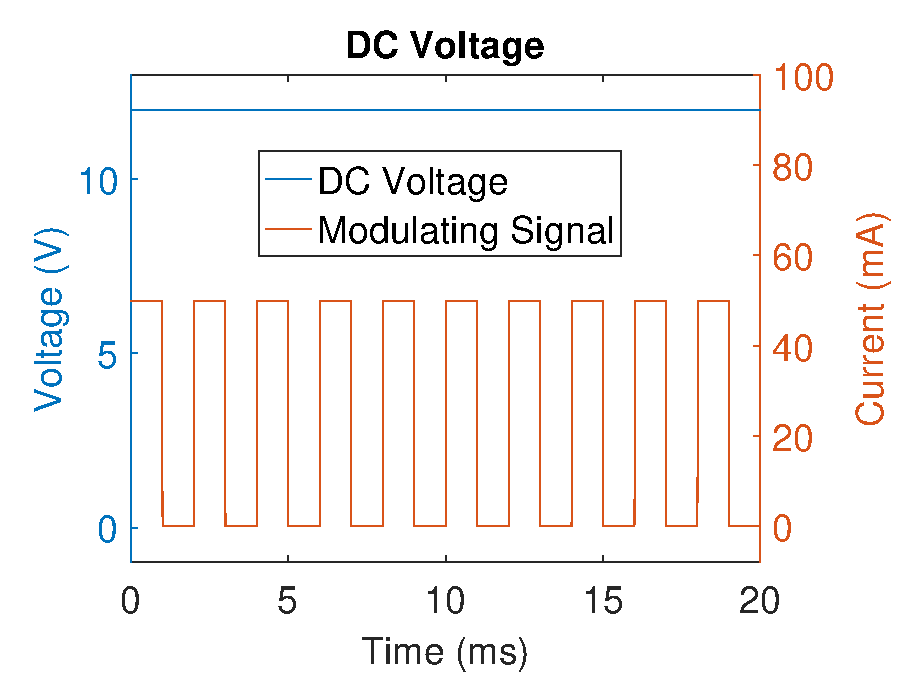
\includegraphics[angle=0,width=0.5\textwidth]{chapters/hardware-chapters/DC/dc-voltage-and-current-example.eps}
  \caption{Voltage of a DC power supply, along with the current of a switching load.}
  \label{fig:dc-voltage-and-current-example}
\end{figure}



This is the ideal way the modulator for an LED must work.
In the next sections, the hardware for the modulator will be explained as well as how the current will be measured to extract the encoded information and finally a testbed will be presented. 





% !TeX root = ../../../../thesis.tex

\subsection{Modulator}

	The task of the modulator is to switch the LED on or off based on the ID that is assigned to the light fixture.
	It is the responsibility of this piece of hardware to translate the ID into the unique current signature.


	The way an LED (Light Emitting Diode) works, is that current has to flow through it in order for it to emit light.
	In other words, an LED is controlled via current, it is not controlled by applying a voltage to it.
	When a certain amount of current flows through the LED, a certain amount of voltage will drop over the LED.

	The easiest way to make an LED emit light, is to put a current limiting resistor in series with a voltage source and an LED.
	A schematic can be seen in \autoref{fig:dc-led-resistor}.
	But there exists no ideal DC power supply.
	Depending on the load, the provided voltage of the power supply may fluctuate.
	Due to the fluctuation of the provided voltage, the LED can start to change in brightness.
	The current that flows through the LED is a function of the voltage over the resistor and the value of the resistor: $I = \frac{U}{R}$.
	So if $U$, the provided voltage, is fluctuating, the current that flows through the LED, $I$, will also fluctuate.
	This causes the brightness of the LED to fluctuate.


	A better way to power an LED, is by using a current source.
	Where an ideal voltage source will always deliver a certain amount of voltage independent of the load, a current source will always deliver a certain amount of current independent of the load.
	If a constant amount of current flows through the LED, the brightness will not fluctuate.
	In \autoref{fig:dc-led-current-source} a schematic can be seen, which shows an example of a current source powering an LED.
	This current source can be toggled on and off via a 0 V or 3.3/5 V signal, coming from a micro-controller, uC in the schematic.


	\begin{figure}[t]
		\centering
		\begin{minipage}[b]{0.3\textwidth}
			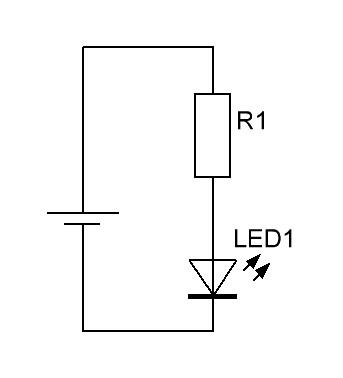
\includegraphics[width=\textwidth]{chapters/hardware-chapters/DC/dc-modulator/dc-led-resistor.jpg}
			\caption{Simplest way to power an LED.}
			\label{fig:dc-led-resistor}
		\end{minipage}
		\hfill
		\begin{minipage}[b]{0.5\textwidth}
			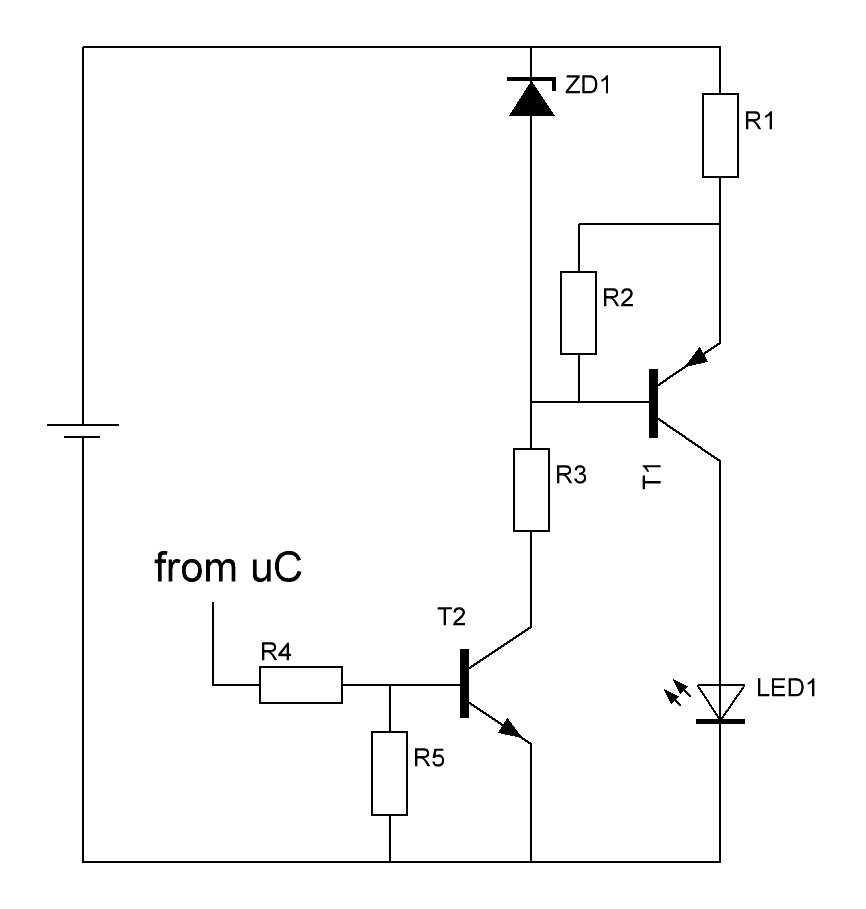
\includegraphics[width=\textwidth]{chapters/hardware-chapters/DC/dc-modulator/dc-led-current-source.jpg}
			\caption{Current source powering an LED.}
			\label{fig:dc-led-current-source}
		\end{minipage}
	\end{figure}

	By using a current source, two benefits can be identified:

	\begin{itemize}
		
		\item Since the current that flows through the LED is constant, the LED will not flicker.

		\item The current source will make sure that the current that is drawn, is either zero or some constant value depending on the bit that is being encoded.
		This will yield a signal with two distinct values.
		When multiple of these signals are aggregated and measured by a smart-meter, the measured signal will also have distinct values.
		This signal will make it easy to decode the information that was encoded by the modulators.

	\end{itemize}

% !TeX root = ../../../../thesis.tex

 \subsection{Current Sampler}

	Now that the hardware is created to translate the IDs of the LEDs into a unique current signature, we also need a way to measure the current.
	The measured current can then be processed by a micro-controller.
	And in turn it can be identified which LEDs are on and which are off.

	In the interest of time the most simple manner was chosen to measure the current for the DC hardware.
	Other options are available for measuring current and they will be discussed in the AC part.
	The most simple way to measure current is by using a series resistor.
	The resistance does not variate and therefore no noise is introduced in the sampled signal.
	The resistor is placed in series between the DC power supply and the LEDs.
	The voltage drop over the resistor is linearly proportional to the current that flows through the resistor, according to Ohm's Law $U = R \times I$.
	If the value of the resistor is chosen such that the maximum voltage will never exceed the rated voltage for a micro-controller, it can be directly measured by the micro-controller's ADC in question.

% !TeX root = ../../../../thesis.tex

\subsection{Testbed}
	\label{subsec:dc-testbed}

	To be able to test all aspects of the system a testbed was created.
	This testbed will allow the testing of the correlation calculations as discussed in \autoref{sec:mapping-problem}, the interference solutions (\autoref{subsec:continuous-method-modulation}), and the performance of the modulator and current-sampler.


	\begin{figure}[ht]
		\centering
		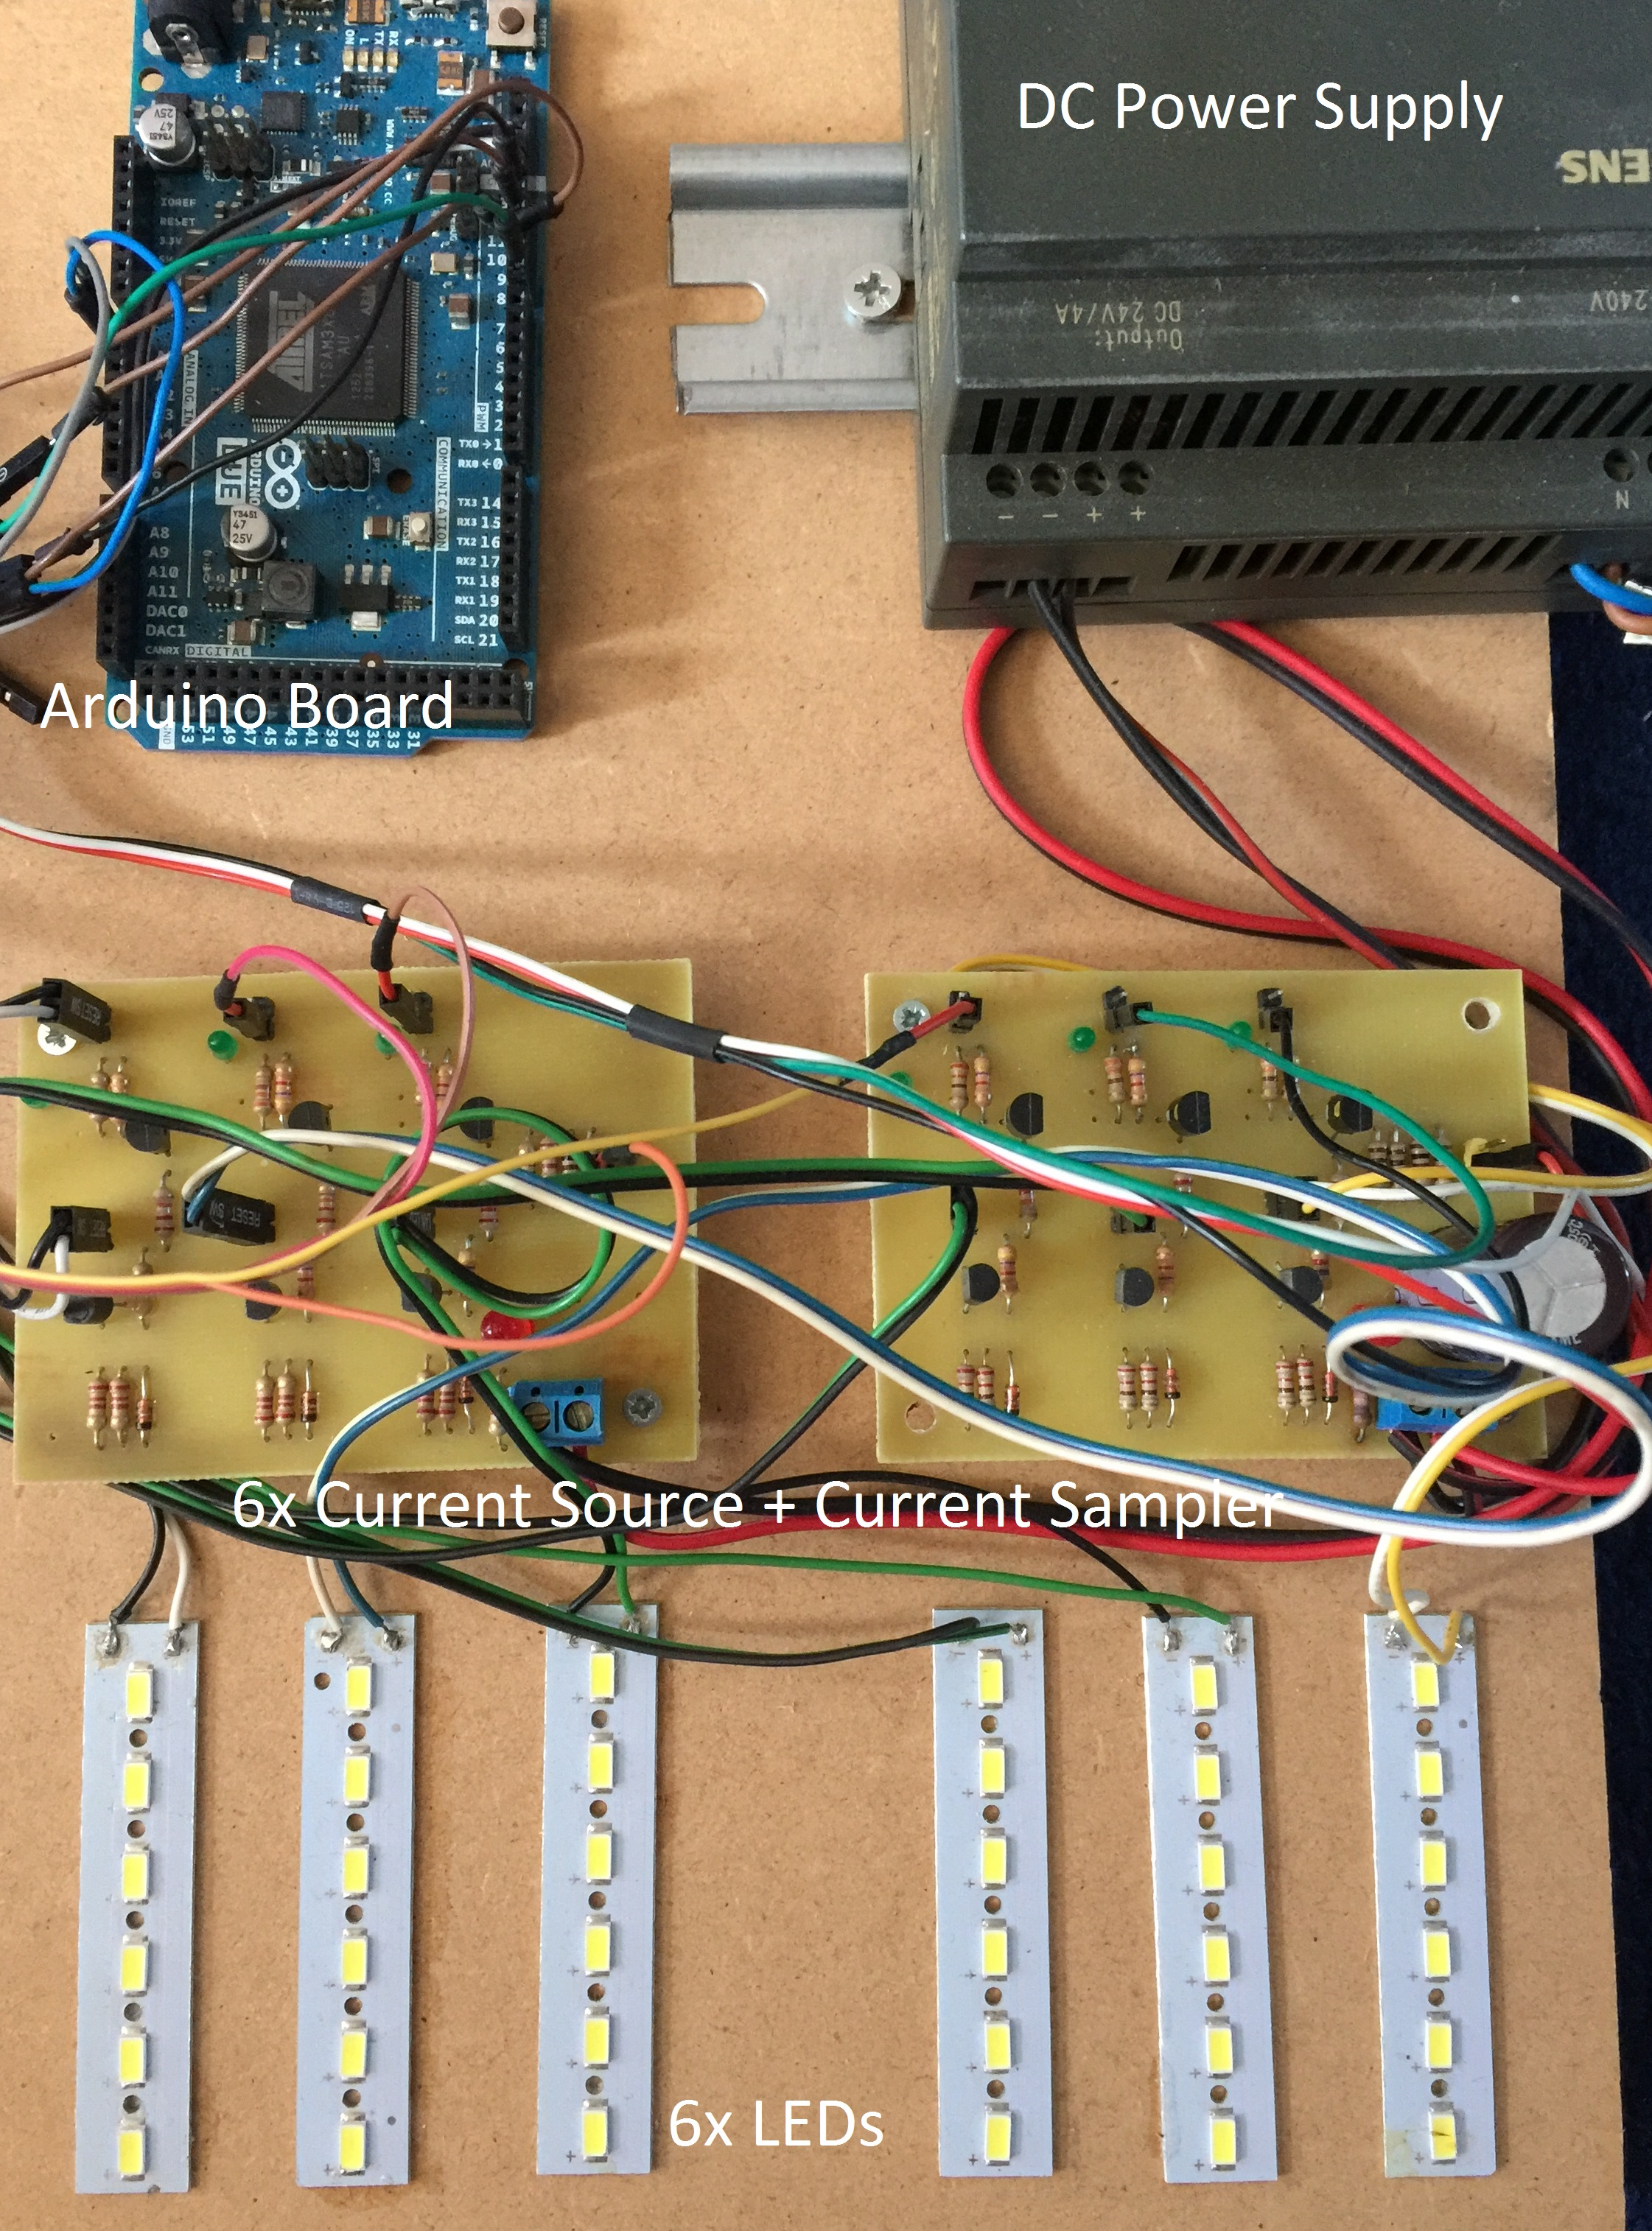
\includegraphics[angle=0,width=0.6\textwidth,height=.9\textheight,keepaspectratio]{chapters/hardware-chapters/DC/dc-test-bed/dc-test-bed-picture.JPG}
		\caption{Picture of the DC testbed, showing the six LED strips, current sources, current sampler and an Arduino board.}
		\label{fig:dc-test-bed-picture}
	\end{figure}

	\begin{figure}[ht]
		\centering
		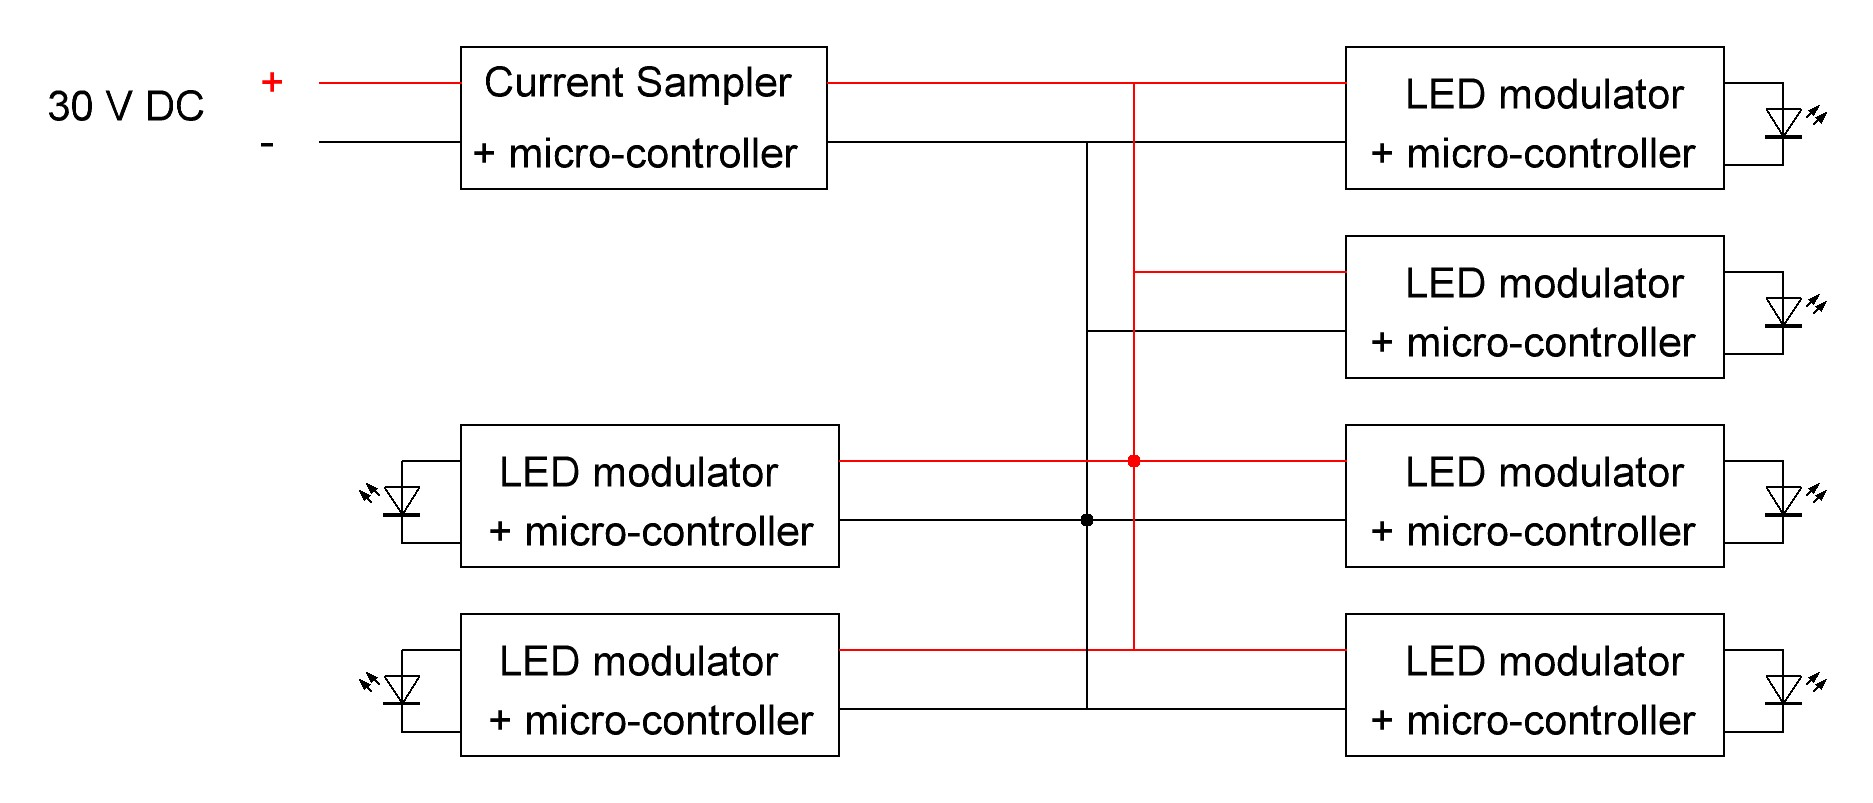
\includegraphics[angle=0,width=1.0\textwidth,keepaspectratio]{chapters/hardware-chapters/DC/dc-test-bed/dc-test-bed-architectural.JPG}
		\caption{Architectural overview of the DC testbed. Six LED modulators are connected in parallel with each other and in series with the current sampler.}
		\label{fig:dc-test-bed-architectural}
	\end{figure}


	The testbed works with a DC power supply and has six individual controllable current sources.
	Each current source powers one LED fixture.
	The testbed itself can be seen in \autoref{fig:dc-test-bed-picture} and an architectural overview of how everything is connected to each other can be seen in \autoref{fig:dc-test-bed-architectural}.


	The aim of the testbed was to use commercial LEDs. 
	The LED fixtures used in this testbed all came from the same commercial LED, which can be found in \cite{commercial-230v-ac-led-aliexpress}.
	A picture of the LED can be seen in \autoref{fig:ac-commercial-230v-ac-led}.
	The strips are taken out of this commercial LED and used individually for this testbed.


	The current is measured by a series resistor and fed to the ADC of a micro-controller.
	The entire schematic of the DC testbed can be found in \autoref{app:dc-test-bed}. 

	The current sources and therefore the LEDs, can be toggled on and off by a micro-controller.
	By toggling the current sources on and off, the current that flows through the series resistor will change accordingly.
	A change of voltage over the series resistor can then be measured by the ADC.

	The measured current from the DC testbed can be seen in \autoref{fig:raw-dc-test-bed-data-short}.
	In this experiment, all six LEDs are modulating with the unique ID that was assigned to each LED.
	The voltage drop over the resistor is measured with the ADC.
	The raw ADC value can be seen on the left y-axis and the calculated aggregated current that is drawn can be seen on the right y-axis.
	From this figure seven distinguishable states can be seen.
	When there are no LEDs on, all LEDs are encoding a `0' data bit, the current is zero.
	When one of the six LEDs is transmitting a `1' data bit, the current jumps to roughly 50 mA.
	When two of the six LEDs are encoding a `1', the current is roughly 100 mA and so on.


	\begin{figure}
		\centering
		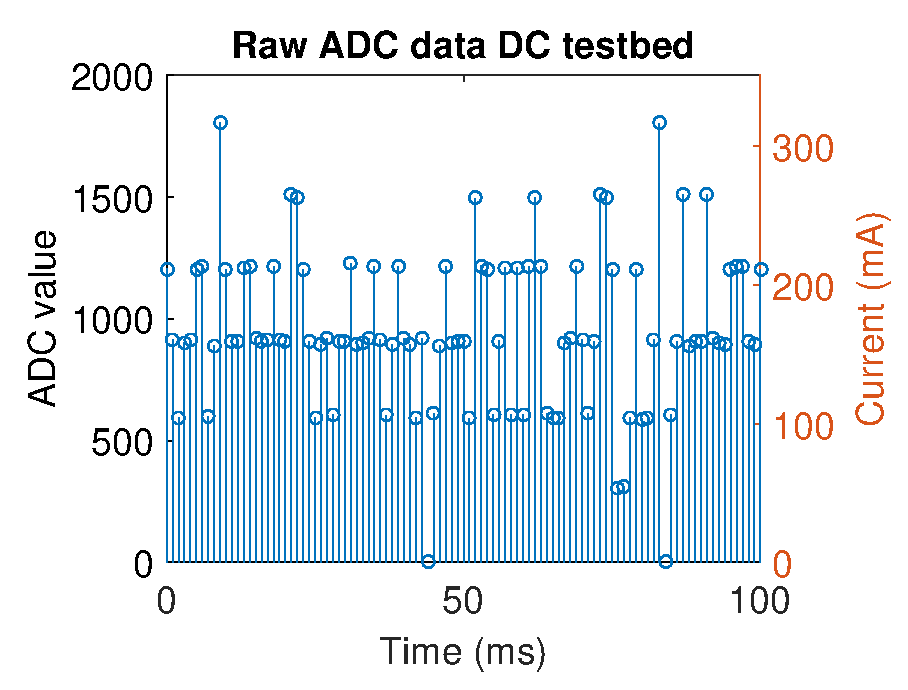
\includegraphics[angle=0,width=0.7\textwidth,keepaspectratio]{chapters/hardware-chapters/DC/dc-test-bed/dc-test-bed-raw-data.eps}
		\caption{Raw current data from the DC testbed with the six LEDs modulating with their unique IDs.}
		\label{fig:raw-dc-test-bed-data-short}
	\end{figure}



	An evaluation of this testbed is done in \autoref{subsec:dc-testbed-eval} where a longer signal will be shown along with correlation data to identify if a certain LED is on, while the other LEDs are modulating and thereby causing interference.













% !TeX root = ../../../thesis.tex

\section{AC Environment}
\label{sec:ac-environment}




The translation from an ID, that is assigned to a light fixture, to a unique current signature is more difficult in an AC environment compared to the DC environment.
This is due to the supplied voltage.
In a DC environment, the voltage is a constant value, but in an AC environment the supplied voltage is a sinusoidal wave.
This means that the voltage will be both positive and negative.
In the Netherlands the AC has an RMS voltage of 230 V and a frequency of 50 Hz.

In the next subsections, we will first describe existing hardware and their limitations.
Then new hardware is proposed to solve the limitations of the existing hardware.
Finally, the AC testbed is showcased.




% !TeX root = ../../../../thesis.tex


\subsection{Modulator}	
\label{subsec:ac-modulator}

The job of the modulator in an AC environment, is the same as in a DC environment.
Just like in the DC environment, when a `0' has to be encoded the current should be zero and when a `1' has to be encoded the current should be some constant value.
The transition between a `0' and `1' should be fast, so that a square wave is created, just like in the DC case.

If the translation is done in this manner, the mapping between the code sequence symbols and the current is clear and the aggregated current drawn by multiple lights will also be a square wave, which will allow for decoding the information.
Next, existing hardware is investigated to see if they can modulate the current draw as ideal square waves.
%if these solutions will translate the IDs into a current draw which is similar to what has just been discussed above. 



\input{chapters/hardware-chapters/AC/ac-modulator/smps-led/smps-led}




	\begin{figure}
		\centering
		\begin{minipage}[b]{0.45\textwidth}
			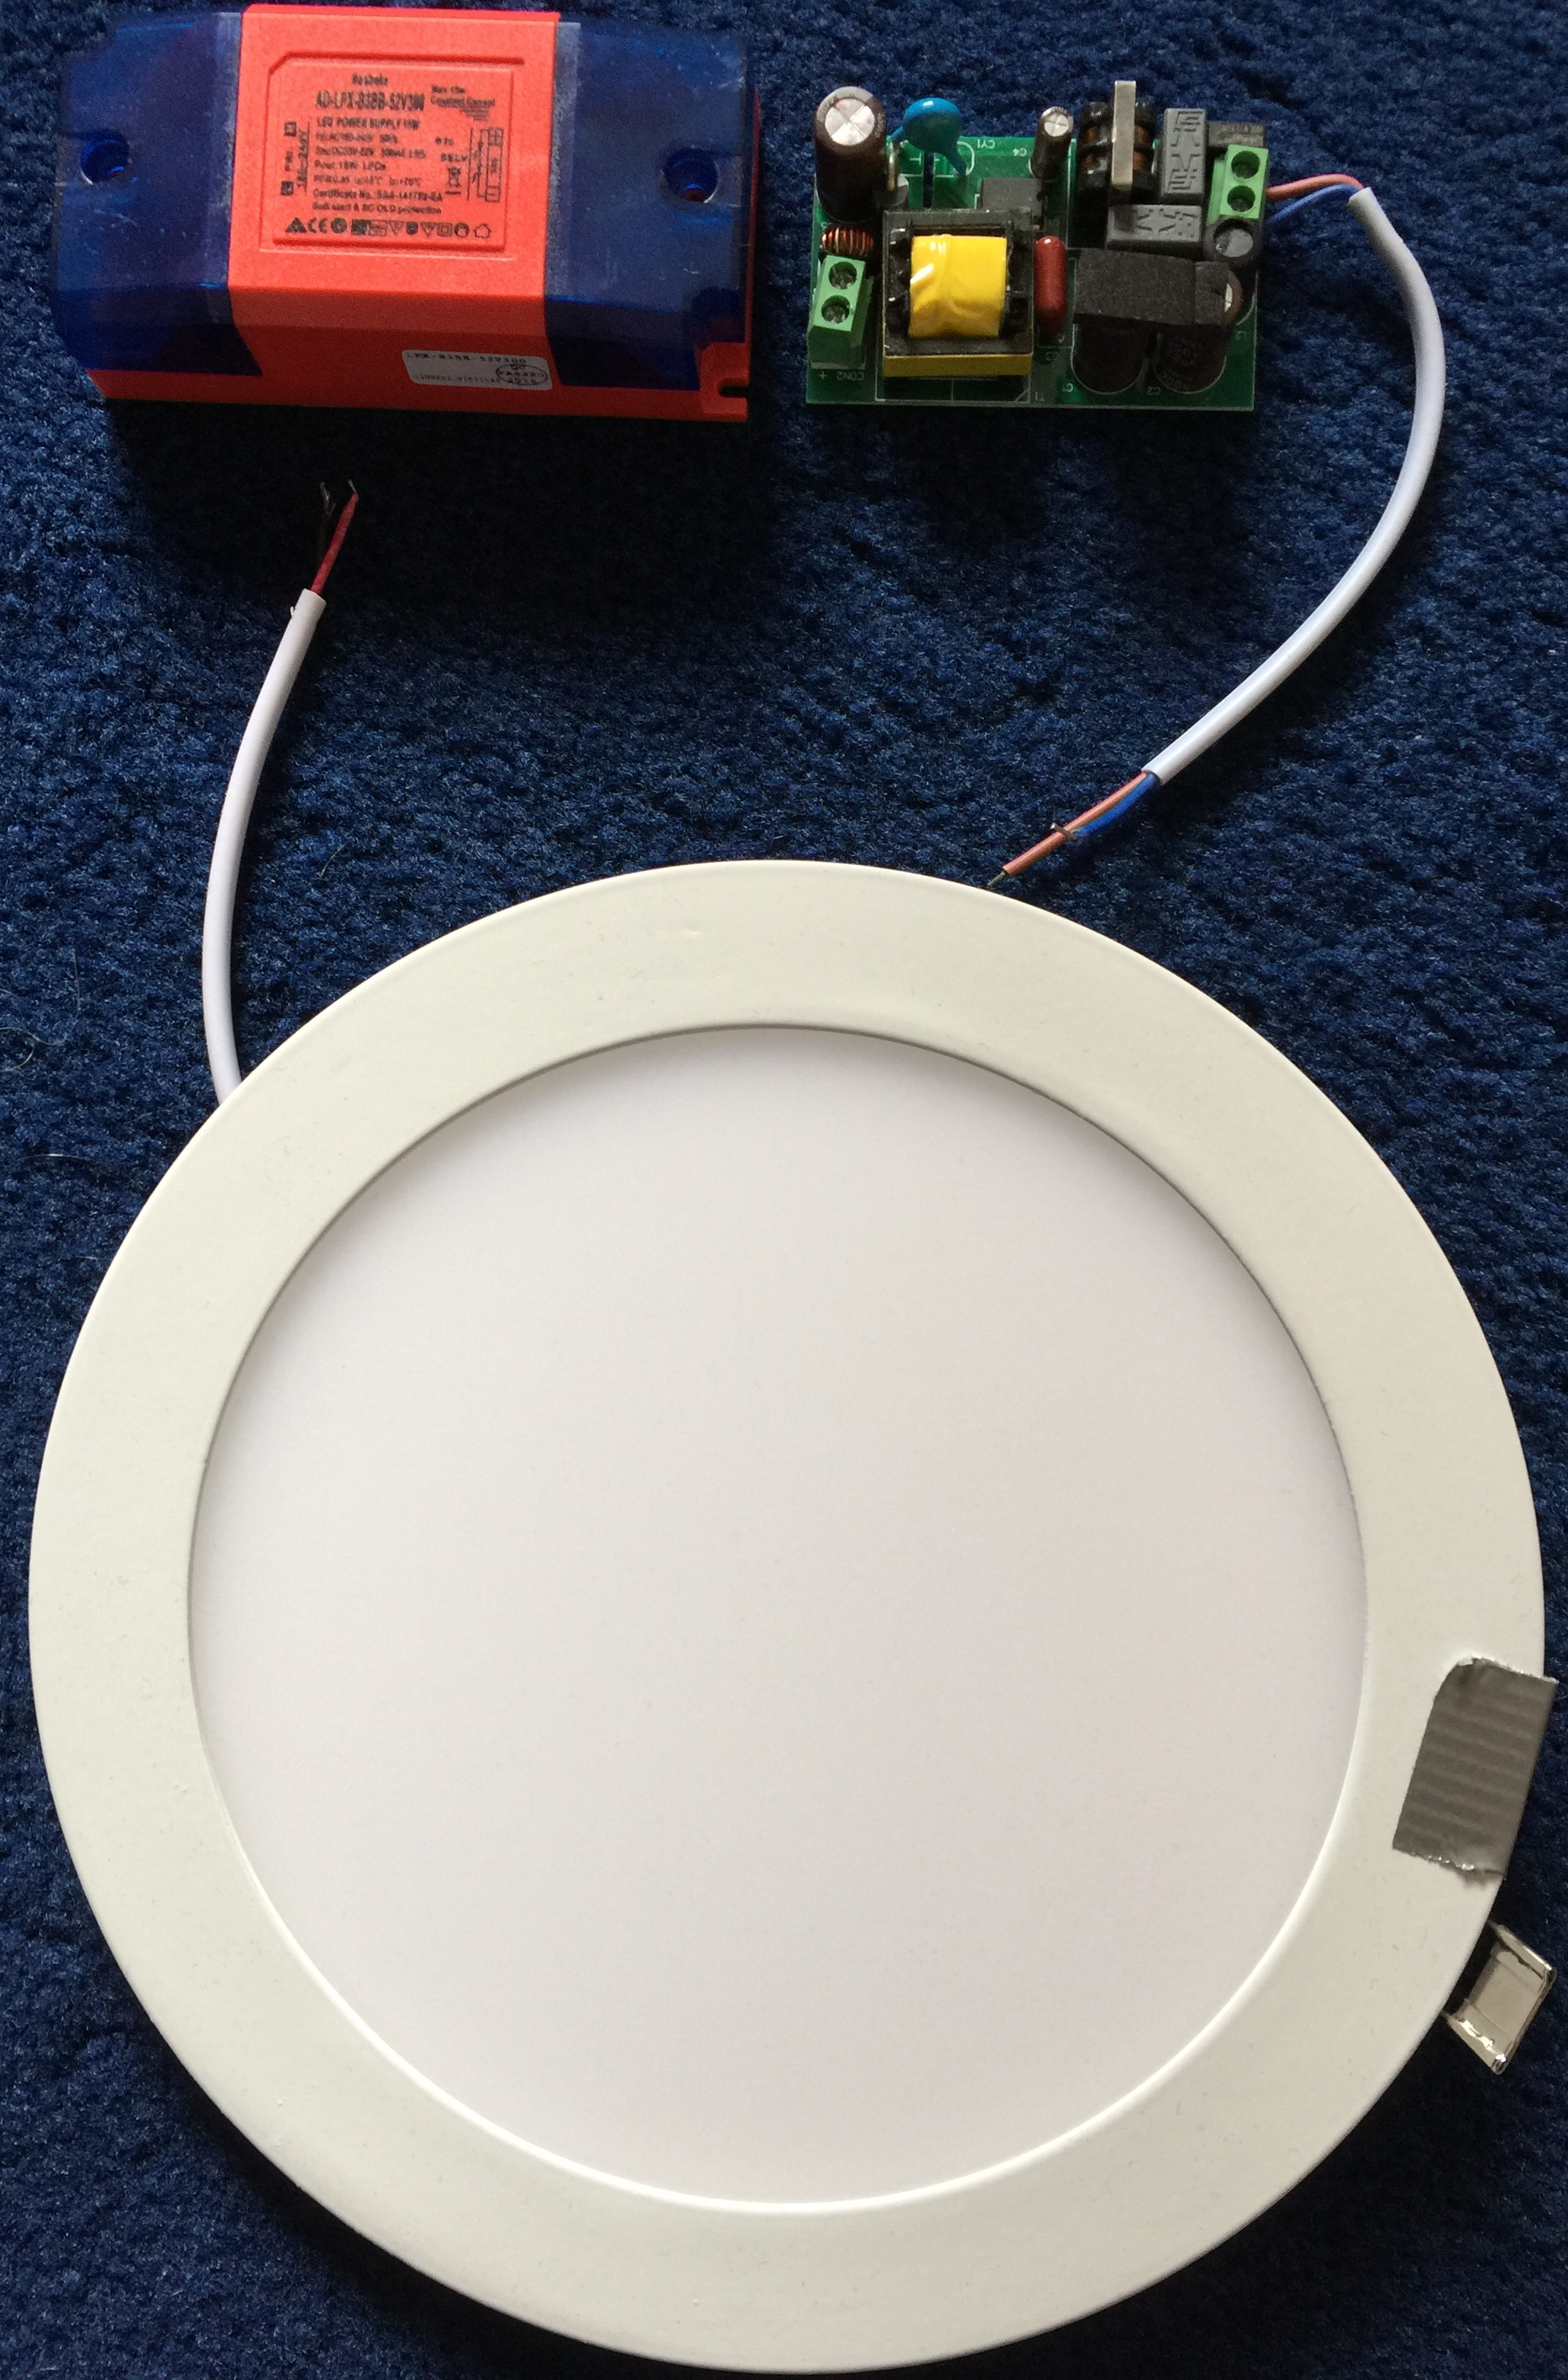
\includegraphics[width=\textwidth]{chapters/hardware-chapters/AC/ac-modulator/smps-led/smps-led-and-smps-picture.jpg}
			\caption{Picture of a commercial LED light fixture with a DC SMPS.}
			\label{fig:ac-smps-led-and-smps-picture}
		\end{minipage}
		\hfill
		\begin{minipage}[b]{0.45\textwidth}
			\centering
			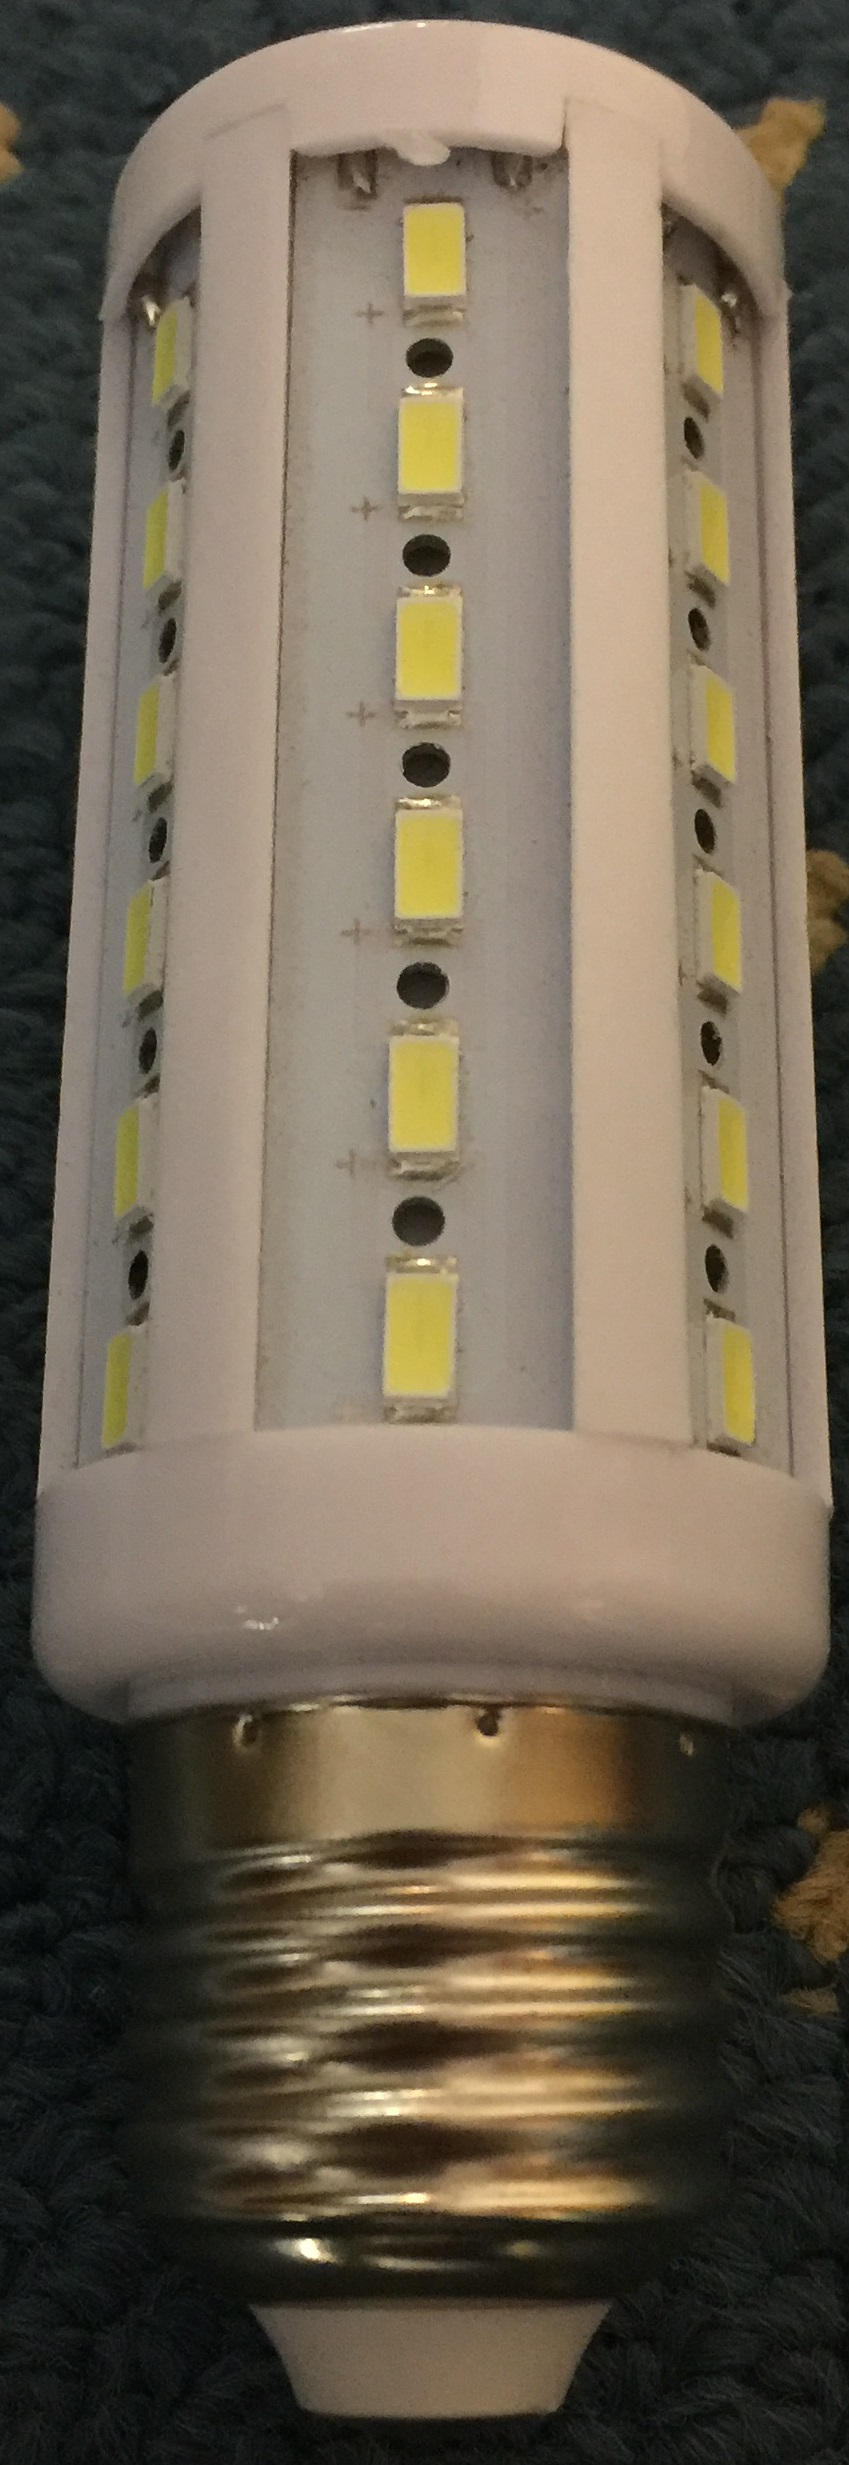
\includegraphics[angle=0,width=0.5\textwidth]{chapters/hardware-chapters/AC/ac-modulator/commercial-230v-ac-led/commercial-ac-led-picture.jpg}
			\caption{Picture of a commercial 230 V AC LED light fixture.}
			\label{fig:ac-commercial-230v-ac-led}
		\end{minipage}
	\end{figure}




\input{chapters/hardware-chapters/AC/ac-modulator/commercial-230v-ac-led/commercial-230v-ac-led}


\input{chapters/hardware-chapters/AC/ac-modulator/custom-hardware/ac-custom-hardware}















% !TeX root = ../../../../thesis.tex


\subsection{Current Sampler}


Now that there exists a solution to encode the ID of an LED into the current draw, as explained in \autoref{subsec:ac-modulator}, it is now time to explore the possibilities to measure the current.
The measured current can then be processed by a micro-controller, and then the status of the LEDs can be determined.


To measure the AC current, first existing solutions were investigated.
One such a product is a `Hall Effect-Based Linear Current Sensor' \cite{hall-ac-current-sensor-datasheet}.
Based on the Hall effect, this sensor outputs a voltage which is proportional to the current that goes through the sensor.
This sensor has the issue that the noise is larger than the voltage signal which is outputted using the provided LEDs.
According to \cite{hall-ac-current-sensor-datasheet}, the highest sensitivity is $185$ mV / A and the noise is rated at $21$ mV.
The commercial LED fixtures which were provided, are rated at $15$ Watts.
With the 230 V AC, this works out to a current of $I = \frac{P}{U} = \frac{15}{230} = 0.065$ A.
At that current the output voltage will be $185 \times 0.065 = 12$ mV.
The noise of the output is $21$ mV, which is almost double the output voltage when one LED is on.
This sensor would not be able to reliably detect one or two LEDs.



Another solution has to be used to overcome the noise problem of the Hall effect sensor.
This solution has two parts: The current sampler itself and a triggering circuit.

The triggering circuit is needed to know when the modulators start and stop encoding the ID.
This will help the smart-meter, by telling it when to start and stop looking for the IDs of the LEDs.
The triggering circuit is the same circuit that was used for the modulator, which was explained in \autoref{subsec:ac-modulator}.
The part which samples the current will be explained next, but first an overview is given of how the different parts of the smart-meter are connected in \autoref{fig:ac-current-sampler-architectural}.
The meter is placed in series with an incoming AC power-line and the LEDs will be connected with the AC output.
The current-sampler forwards information about the current draw to a micro-controller for processing.
And the triggering circuit detects when the voltage is high enough for modulation for the LEDs. 


\begin{figure}[h]
	\centering
	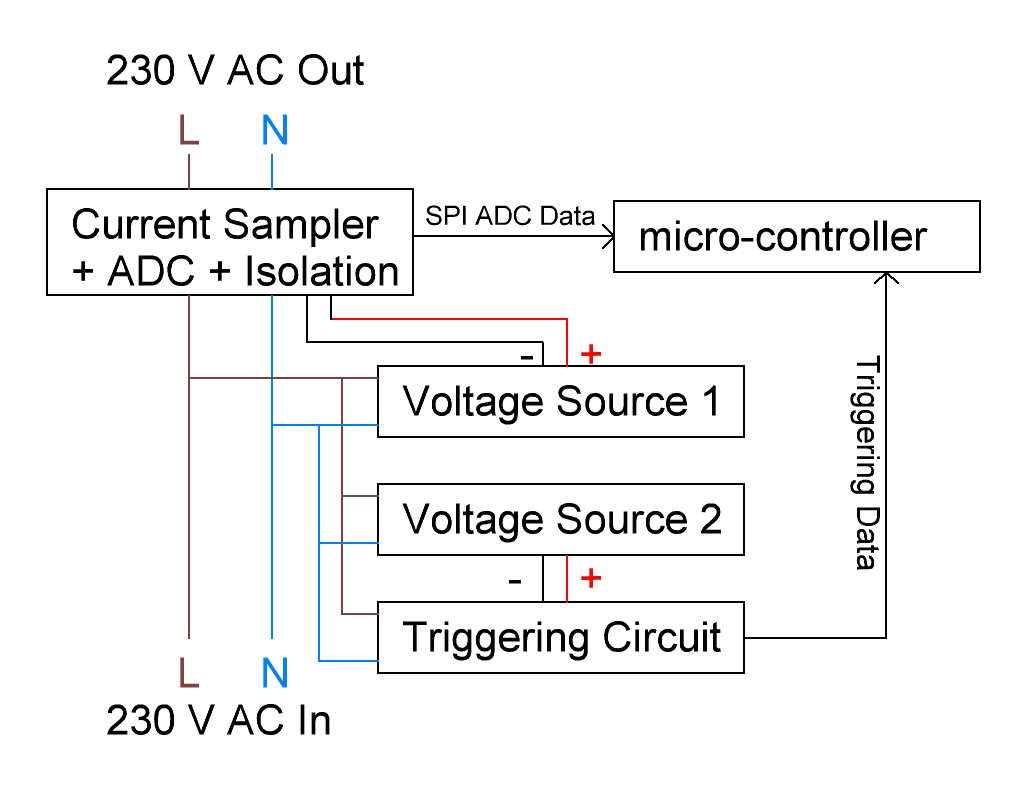
\includegraphics[angle=0,width=0.7\textwidth,keepaspectratio]{chapters/hardware-chapters/AC/ac-current-sampler/ac-current-sampler-architectural.JPG}
	\caption{Architectural overview of the AC current sampler.}
	\label{fig:ac-current-sampler-architectural}
\end{figure}


For the current-sampler itself a resistor will be used, since this approach ensures that no noise will be introduced to the sampled current signal.
As could be seen from \autoref{fig:custom-modulator-current-source}, the current that flows is both positive and negative, due to the nature of the AC that is used.
This means that the voltage that is measured over the resistor will also be positive and negative.
An ADC (Analog-to-Digital Converter) cannot measure a negative voltage.
So the voltage over the resistor is summed with another voltage to ensure that the ADC will always measure a positive voltage.
This other voltage comes from a reference voltage IC \cite{lm336z-ref-voltage-datasheet}, which outputs a very stable reference voltage often used in scenarios where an ADC is used to measure analog signals.

At this point the ADC is measuring the voltage over a resistor which is in series with the ground (N) or phase (L) of the 230 V AC.
For safety reason the ADC must now be electrically isolated from the micro-controller, such that no harm can come from even touching the micro-controller.
To this end, an SPI isolating chip was used \cite{iso7241m-spi-isolator-datasheet} to electrically isolate the SPI signals between the ADC and the micro-controller.




This solution to sample current with an external ADC can sample the current with an high frequency ($> 10$ kHz) with no noise introduced in the signal.
The full schematic of the current sampler can be found in \autoref{app:custom-current-sampler-schematic}.





% !TeX root = ../../../../thesis.tex


\subsection{Testbed}
\label{subsec:ac-testbed}

\begin{figure}[ht]
	\centering
	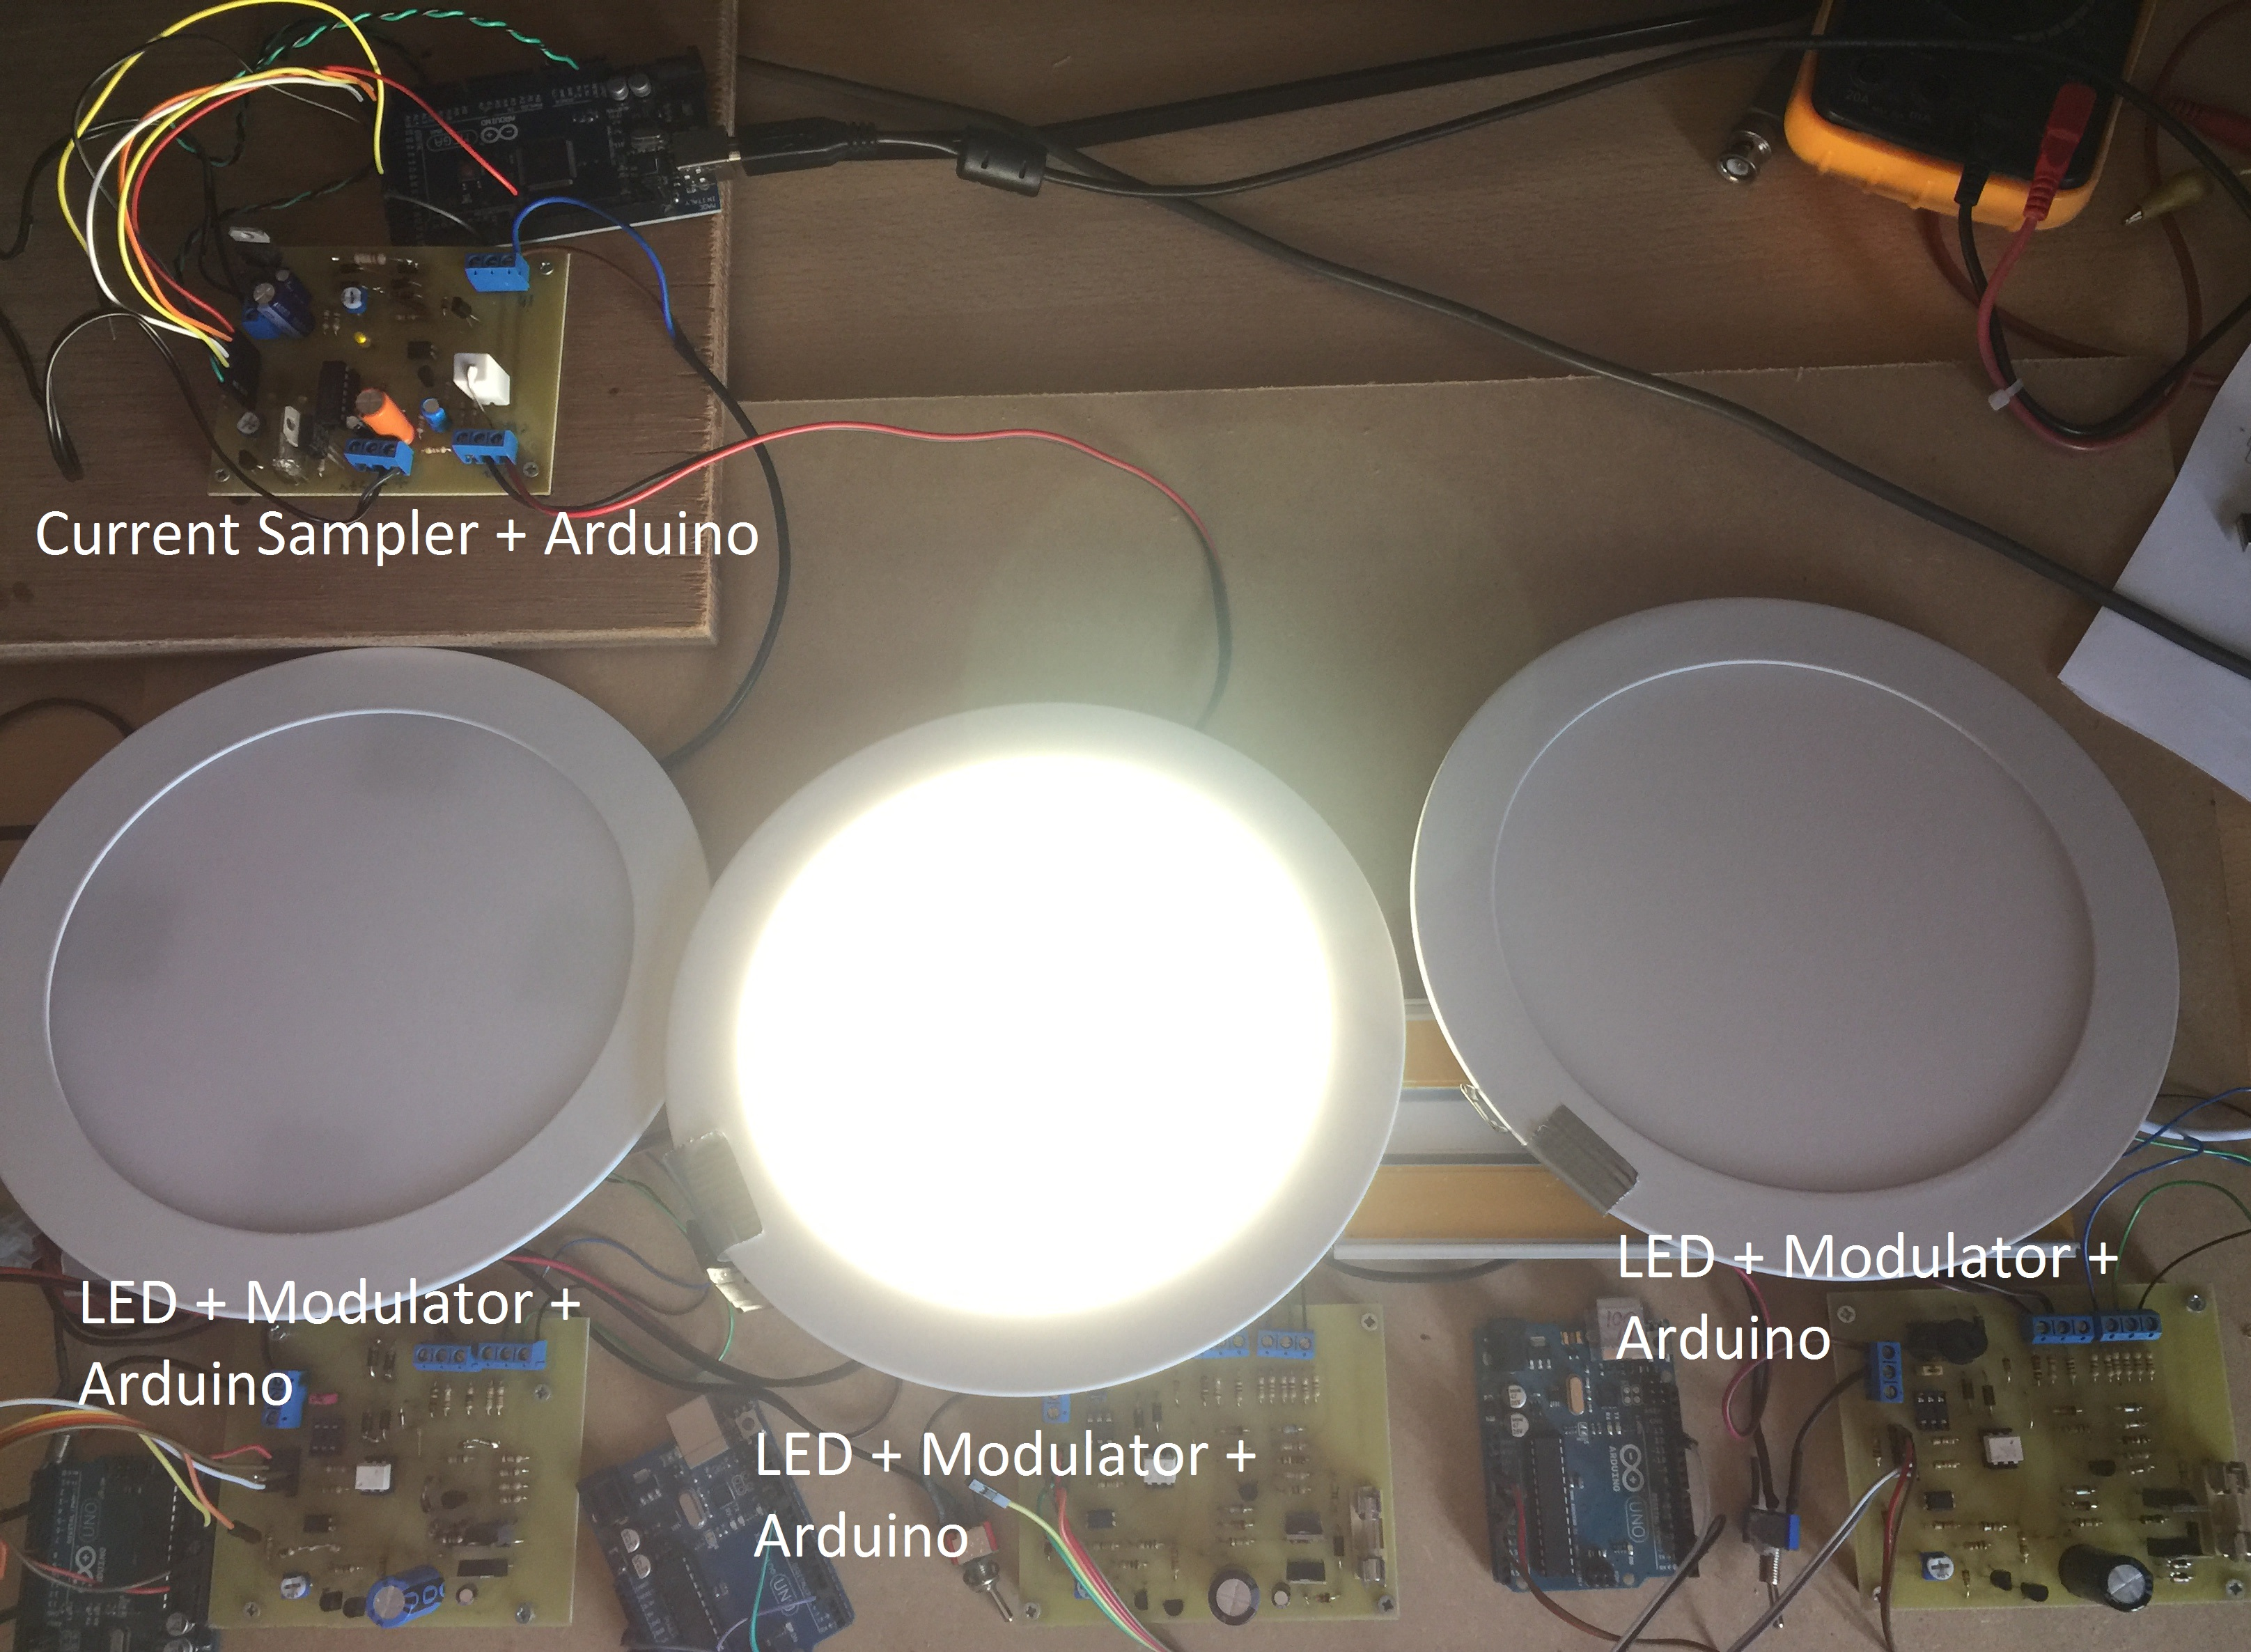
\includegraphics[angle=0,width=\textwidth,height=.9\textheight,keepaspectratio]{chapters/hardware-chapters/AC/ac-test-bed/ac-test-bed-picture}
	\caption{Picture of the AC testbed, consisting of three modulators each connected to three commercial LEDs. The modulators are controlled via three separate Arduino boards. Finally there is the current sampler with its own Arduino board.}
	\label{fig:ac-test-bed-picture}
\end{figure}



An overview of the AC testbed can be found in \autoref{fig:ac-test-bed-architectural-overview} and a picture of the actual testbed itself can be seen in \autoref{fig:ac-test-bed-picture}.
In the testbed three commercial LEDs are used which are powered by the custom modulators as explained in \autoref{subsec:ac-modulator}.
Arduino boards are controlling the modulators.
The modulators are connected in parallel. 
And the custom current-sampler is connected in series to measure the current and decode the information that the modulators encode into the current draw.
The custom current-sampler has its own Arduino board to process the current signal.
All Arduino board are stand-alone, and are not connected to each other in any way.


\begin{figure}[t]
	\centering
	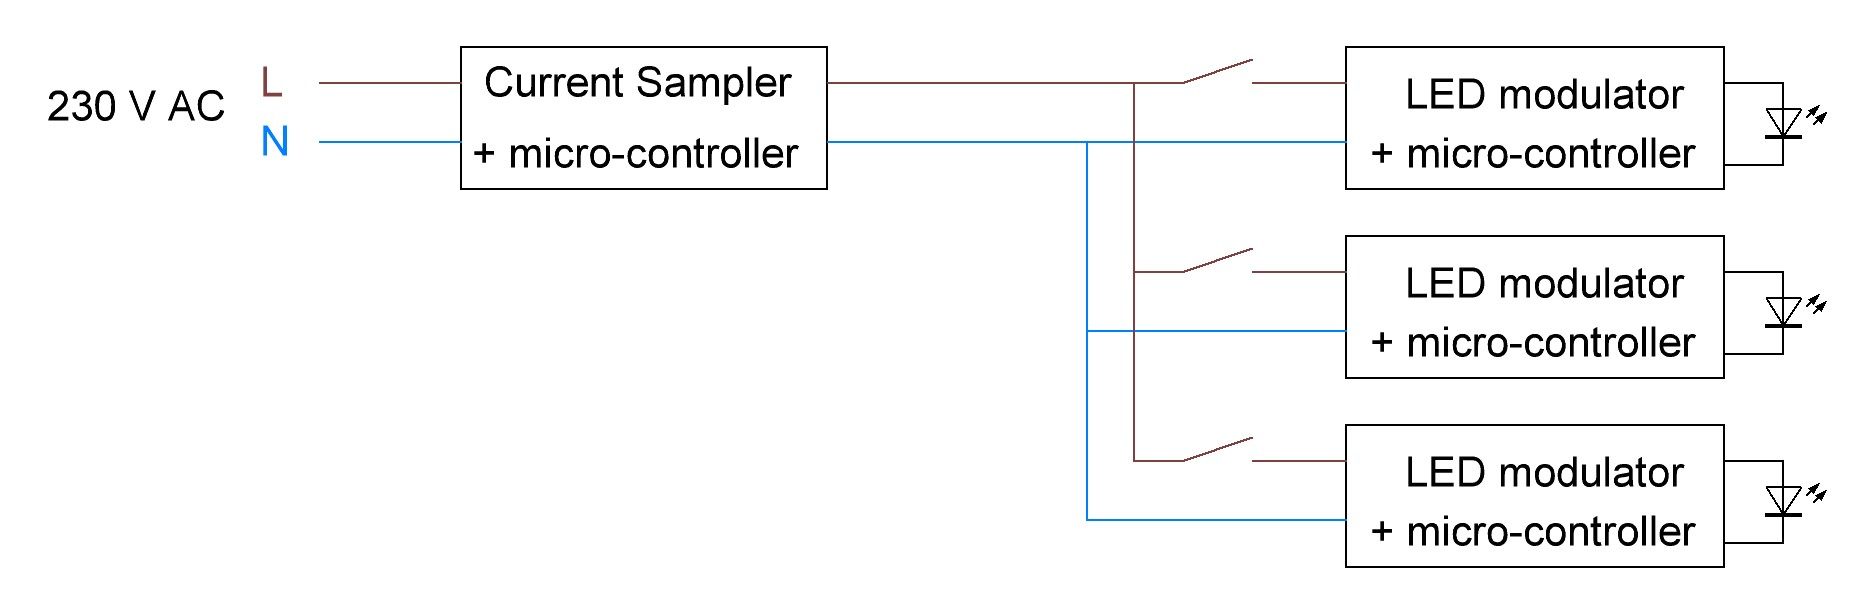
\includegraphics[angle=0,width=0.9\textwidth,keepaspectratio]{chapters/hardware-chapters/AC/ac-test-bed/ac-test-bed-architectural.JPG}
	\caption{Architectural overview of the AC testbed. Three LED modulators, with switches to turn the LED on and off, are connected in parallel with each other and in series with the current sampler.}
	\label{fig:ac-test-bed-architectural-overview}
\end{figure}



In \autoref{fig:raw-ac-testbed-adc-data-testbed} the raw data that is collected by the smart-meter can be seen.
The current signal is shown here alongside the trigger output.
In the raw data the charging peaks of the capacitor can be seen at timestamps: 5, 15 and 25 ms. %of the non-disturbing voltage source
Note that these peaks indeed do not interfere with the modulated data.
The modulated data and the charging peaks can be filtered out by the micro-controller with the help of the triggering circuits logical output.
As discussed in \autoref{subsec:ac-modulator}, the time that is available for modulation is 8 ms in a 10 ms period.
Depending on the length of the ID $L$ and the modulation frequency $f$, it can happen that this window of 8 ms is too small to encode the entire ID.
In this case, the remaining bits of the ID which could not fit inside the first 8 ms window, will be transmitted in the next window.
An evaluation with this testbed will be done in \autoref{subsec:ac-evaluation}.



\begin{figure}[ht]
  \centering
  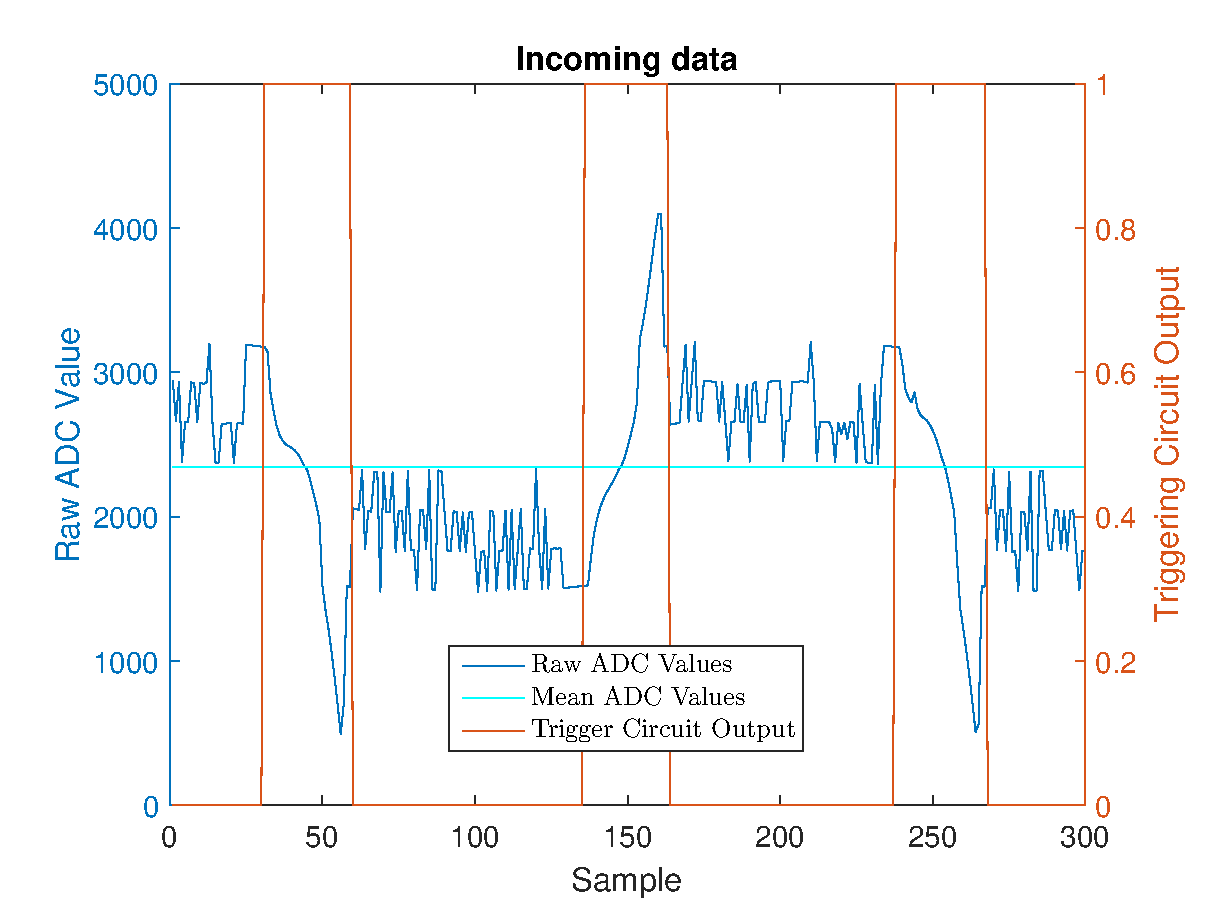
\includegraphics[width=0.7\textwidth]{chapters/evaluation-chapters/hardware/ac/raw-ac-testbed-adc-data.eps}
    \caption{Incoming data to the AC current sampler. The raw ADC values are plotted as well as the triggering circuit output.}
  \label{fig:raw-ac-testbed-adc-data-testbed}
\end{figure}



% CHAPTERS ... For instance: History/Prior Work, Design/Implementation, Experiments
%\chapter{CHAPTER TITLE}
\label{chp:CHAPTERTITLE}
INTRODUCTION TEXT TO THIS CHAPTER IN WHICH ALL SECTIONS ARE DESCRIBED ROUGHLY (1 SENTENCE EACH).

This chapter describes the ... In Section~\ref{sec:SECTIONTITLE}, examples are given of how to use tables and figures in MSc theses.

\section{SECTION TITLE}
\label{sec:SECTIONTITLE}

Every caption of a table (or figure) should start with a capital letter, and should end with a period. References to tables are given with a capital letter for table, as in ``(see Table~\ref{tab:EXAMPLETABLE})'' or ``in Table~\ref{tab:EXAMPLETABLE}, ...''.

\begin{table}[htb]
\centering
\begin{tabular}{|l|c|r|}
\hline % horizontal line
left aligned & centred & right aligned \\
\hline \hline
12           & 34      & 56            \\
\hline
\end{tabular}
\caption{Complete sentence describing the tabular data.}
\label{tab:EXAMPLETABLE}
\end{table}

References to figures are given with a capital letter for figure, as in ``(see Figure~\ref{fig:EXAMPLEFIGURE})'' or ``in Figure~\ref{fig:EXAMPLEFIGURE}, ...''.

\cite{b}
\cite{a}

\begin{figure}[htb]
% most GNUplot figures need to be rotated, width should be the same throughout the complete document, and no extension is needed

\includegraphics[angle=180,width=\textwidth]{pics/TUD_logo_zw}
\caption{Complete sentence describing the figure thoroughly.}
\label{fig:EXAMPLEFIGURE}
\end{figure}



% CONCLUSIONS AND FUTURE WORK
% !TeX root = ../thesis.tex

\chapter{Conclusions and Future Work}
\label{chp:conclusionsandfuturework}

	\section{Conclusions}


	The aim of this thesis is to find out if lights could be identified as being on or off, through the current signature, with the help of VLC and a single smart-meter.
	CDMA codes have been investigated and compared to see which is the best suited for this scenario.
	Two solutions have been discussed to overcome the interference problem that comes with these types of codes.
	When these codes were understood and made usable in software simulations, two practical testbed were developed, for DC and AC, in order to experiment with.
	When the correct codes are used dependent on the size of the system, each individual light in each testbed could be successfully identified as being on or off in a timely manner.
	For larger systems a simulation was performed which shows that there can be made a trade-off between time and accuracy. 
	But the simulation showed that even with a high accuracy, the lights could still be identified in a timely manner.
	%As the testbed only represents a case where only these lights were connected, there is more work to be done when for instance there are also other appliances connected.






\section{Future Work}


This work is only the first step to disaggregate which lights are on and off.
There remains more work to be done, below there are ideas for future work.

	\subsection{Power Limiting Capacitor}

	The solution of using a capacitor in order to limit the power dissipated in the current source, introduced in \autoref{subsubsec:current-source} can be further investigated.
	In particular what the drawbacks or benefits the phase-shifting of current has.
	And if the triggering circuit will still function properly or what the modifications are that need to be made in order for this scheme to work properly.


	\subsection{Other Appliances}

	As the testbeds represents a case where only these lights were connected, the question rises: What will happen when other appliances are connected ?
	These could for example be an incandescent light bulb or a refrigerator.
	To answer that question sample data from \cite{kolter2011redd} could be taken to represent some household appliances and added with the data of the modulation shown from the testbeds.
	Then signal filtering techniques could be performed to try and filter the signal from the modulating lights, given the fact that we know that these lights operate at a certain constant frequency.


	\subsection{Dimming Lights}

	LEDs can be often too bright for a persons liking, so the lights are dimmed.
	Dimming of an LED can be done in two ways: PWM, by lowering the duty cycle and so less power is dissipated by the LED or by limiting the current that flows through the LED.
	Since the LEDs are modulating via an OOK scheme, PWM cannot be used so instead current limiting must be done in order to dim the lights.
	But the CDMA codes are designed to work with each transmitter or LED has the same amplitude or in this case the same current.
	By dimming the LED and changing the current the codes may not work anymore.
	A solution for this can be that each LED will have multiple dimming levels and that for each dimming level other frequencies are used to modulate at.
	A filter can then be used to filter between these LEDs which all have the same amplitude.



	\subsection{Transmitting Data}

	With the current state of this system the LEDs can be identified as being on or off by detecting if their unique code is present or not.
	This can be seen as transmitting data, namely one bit, if the LED is on or off.
	If the LED needs to send other data about the status of the light two approaches can be thought of: 


	\begin{itemize}
		\item The unmodified code assigned to the light will be transmitted for the data-bit `0' and the negation of the code will be transmitted for the data-bit `1'. 
		This gives a problem with the definition of the cross-correlation, which is defined only for the unmodified codes. 
		When the negation of the codes is also used, the cross-correlation between the LEDs that are transmitting is no longer bounded by the mathematical formula and all the calculation on how many LEDs can transmit at the same time can no longer be used with these codes.
		It can be investigated if other codes do have a cross-correlation definition where the negation of the codes is also taken into consideration.

		\item Assign two unique codes from the same set to each light. 
		The lights will send the first code for the data-bit `0' and the second code for the data-bit `1'.
		Since the cross-correlation is defined for the codes from the same set this solution should not yield any problems.
		But further investigation may be required to see if this is a viable solution.
	\end{itemize}


	














% BIBLIOGRAPHY
%#define SORTED 1
\bibliographystyle{bib/latex8}
\bibliography{bib/mycollection}

\appendix


% !TeX root = ../../../thesis.tex

\chapter{DC Testbed Schematic}
\label{app:dc-test-bed-schematic}

\begin{figure}[htb]
	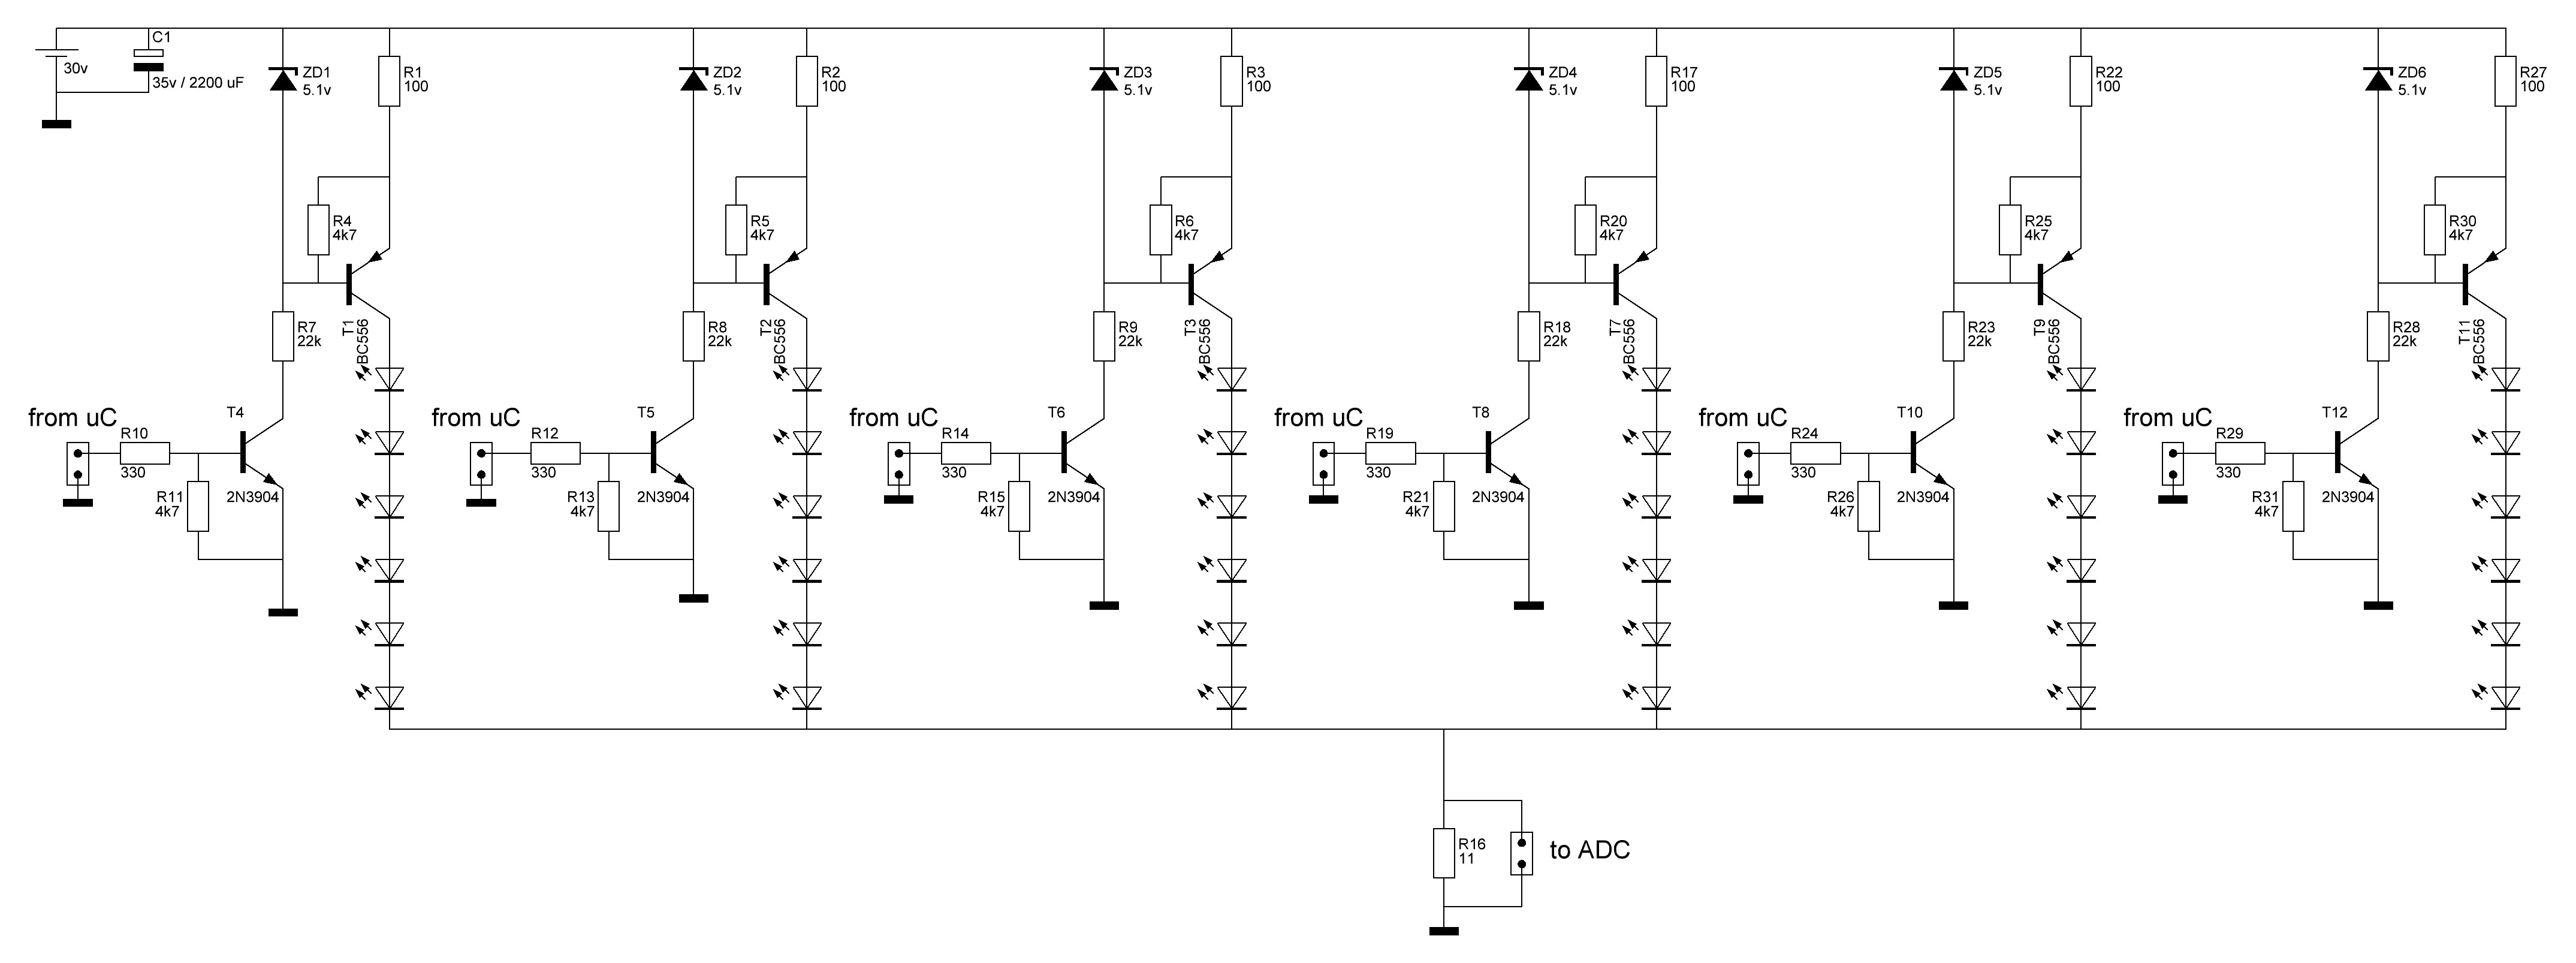
\includegraphics[angle=90,width=\textwidth,height=\textheight,keepaspectratio]{chapters/appendix/dc-test-bed/dc-test-bed-schematic.jpg}
	\caption{Schematic of the DC testbed, to modulate six individual LEDs and measure the combined current.}
	\label{fig:dc-test-bed-schematic}
\end{figure}



% !TeX root = ../../../thesis.tex

\chapter{Modified 230 V AC LED Schematic}
\label{app:commercial-230v-ac-modified-schematic}

In this chapter, the schematic of the original and modified circuit of a commercial 230 V AC LED can be found in \autoref{fig:commercial-230v-ac-modified-schematic}.
The relevant datasheets for parts used can be found in: \cite{4n35-optocoupler-datasheet}, \cite{mth6n60-n-power-fet-datasheet} and \cite{mje13009g-npn-power-transistor-datasheet}.




\begin{figure}[htb]
	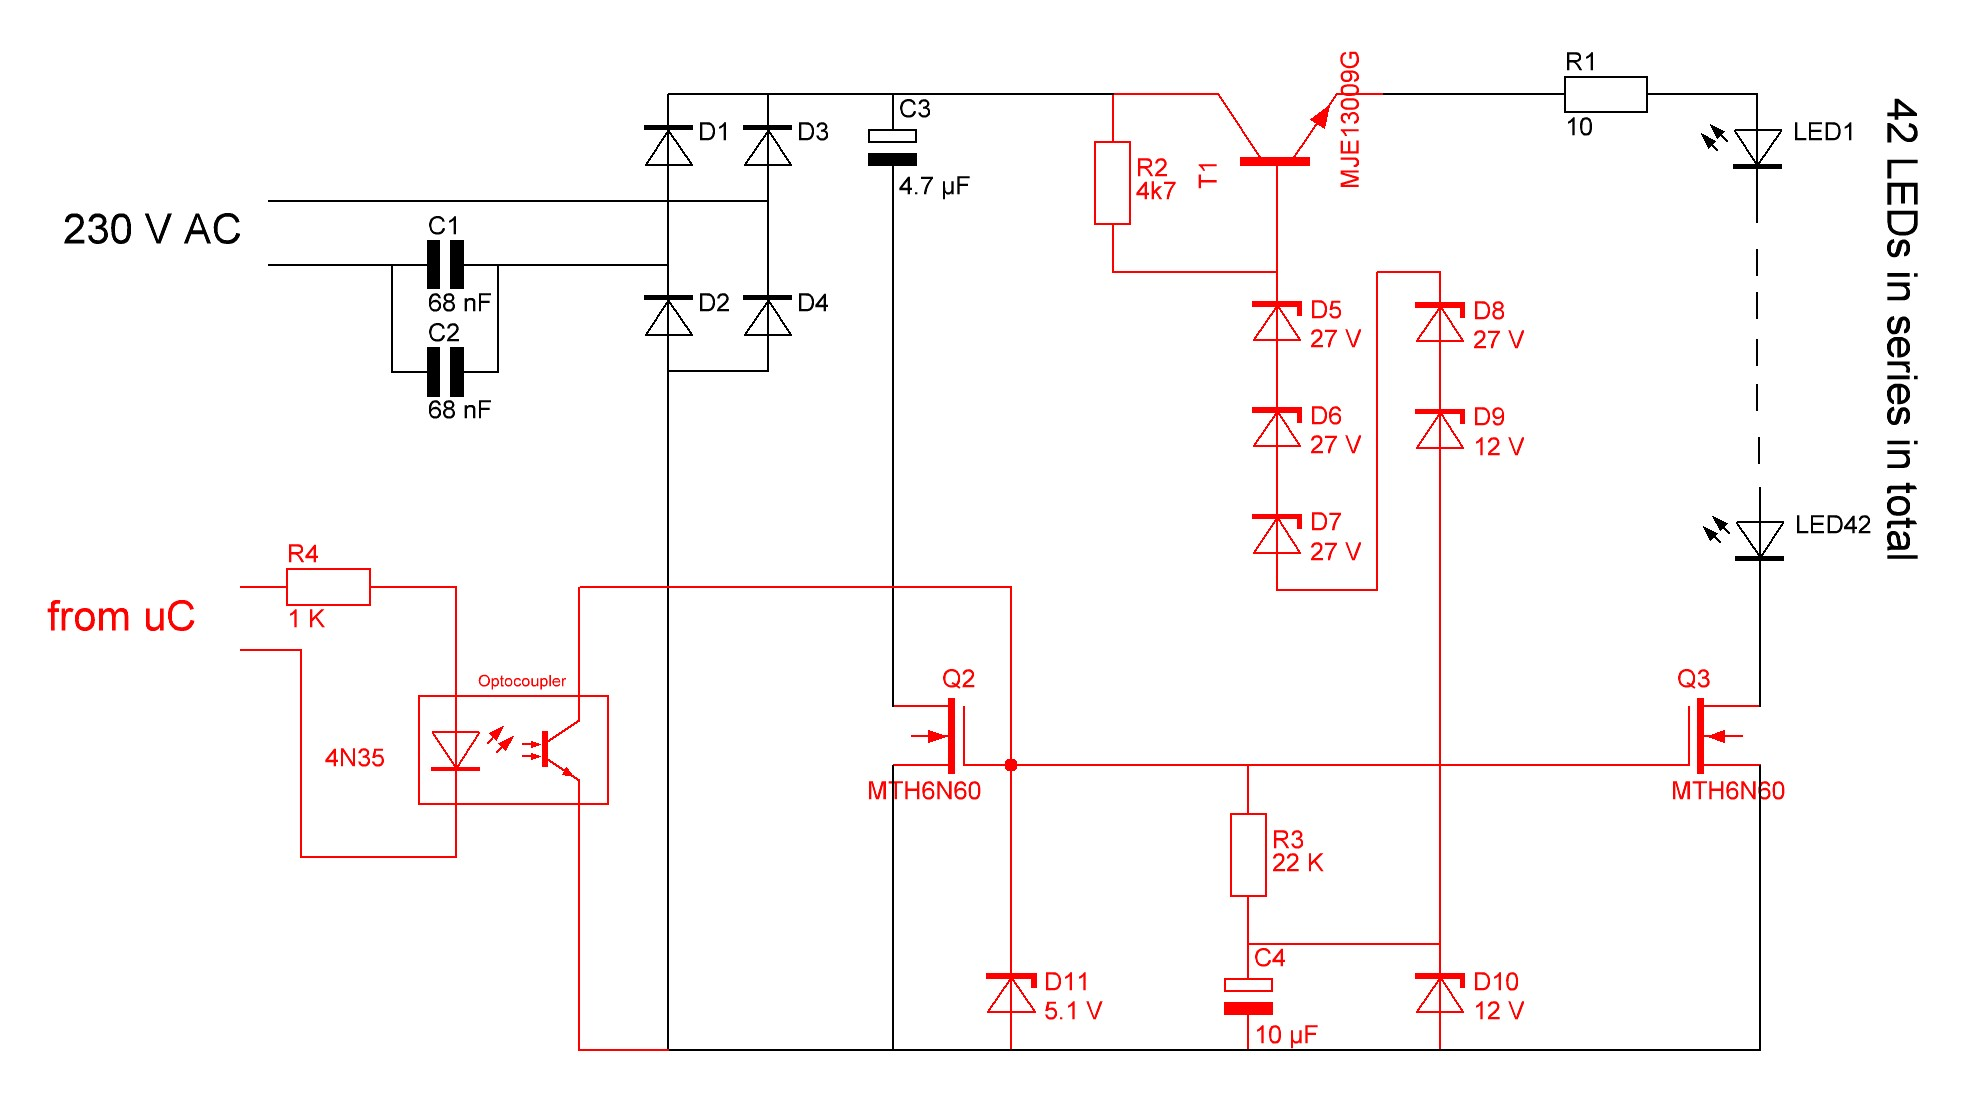
\includegraphics[angle=90,width=\textwidth,height=.9\textheight,keepaspectratio]{chapters/appendix/commercial-230v-ac-modified-schematic/commercial-230v-ac-modified-schematic.jpg}
	\caption{Schematic of the modified commercial 230 V AC LED. Everything in black is from the original schematic. Everything in red is added in order to modulate the LED safely with a microprocessor.}
	\label{fig:commercial-230v-ac-modified-schematic}
\end{figure}


% !TeX root = ../../../thesis.tex

\chapter{Custom LED Modulator Schematic}
\label{app:custom-led-modulator-schematic}

In this chapter, the schematic of the LED modulator can be found in \autoref{fig:custom-led-modulator-schematic}.
The relevant datasheets for parts used, can be found in: \cite{lm7805-vr-datasheet}, \cite{2n7000-n-fet-datasheet}, \cite{sfh617a-optocoupler-datasheet}, \cite{h11l1-optocoupler-datasheet}, \cite{buz80-n-fet-datasheet} and \cite{2n3904-npn-transistor-datasheet}.


\begin{figure}[htb]
	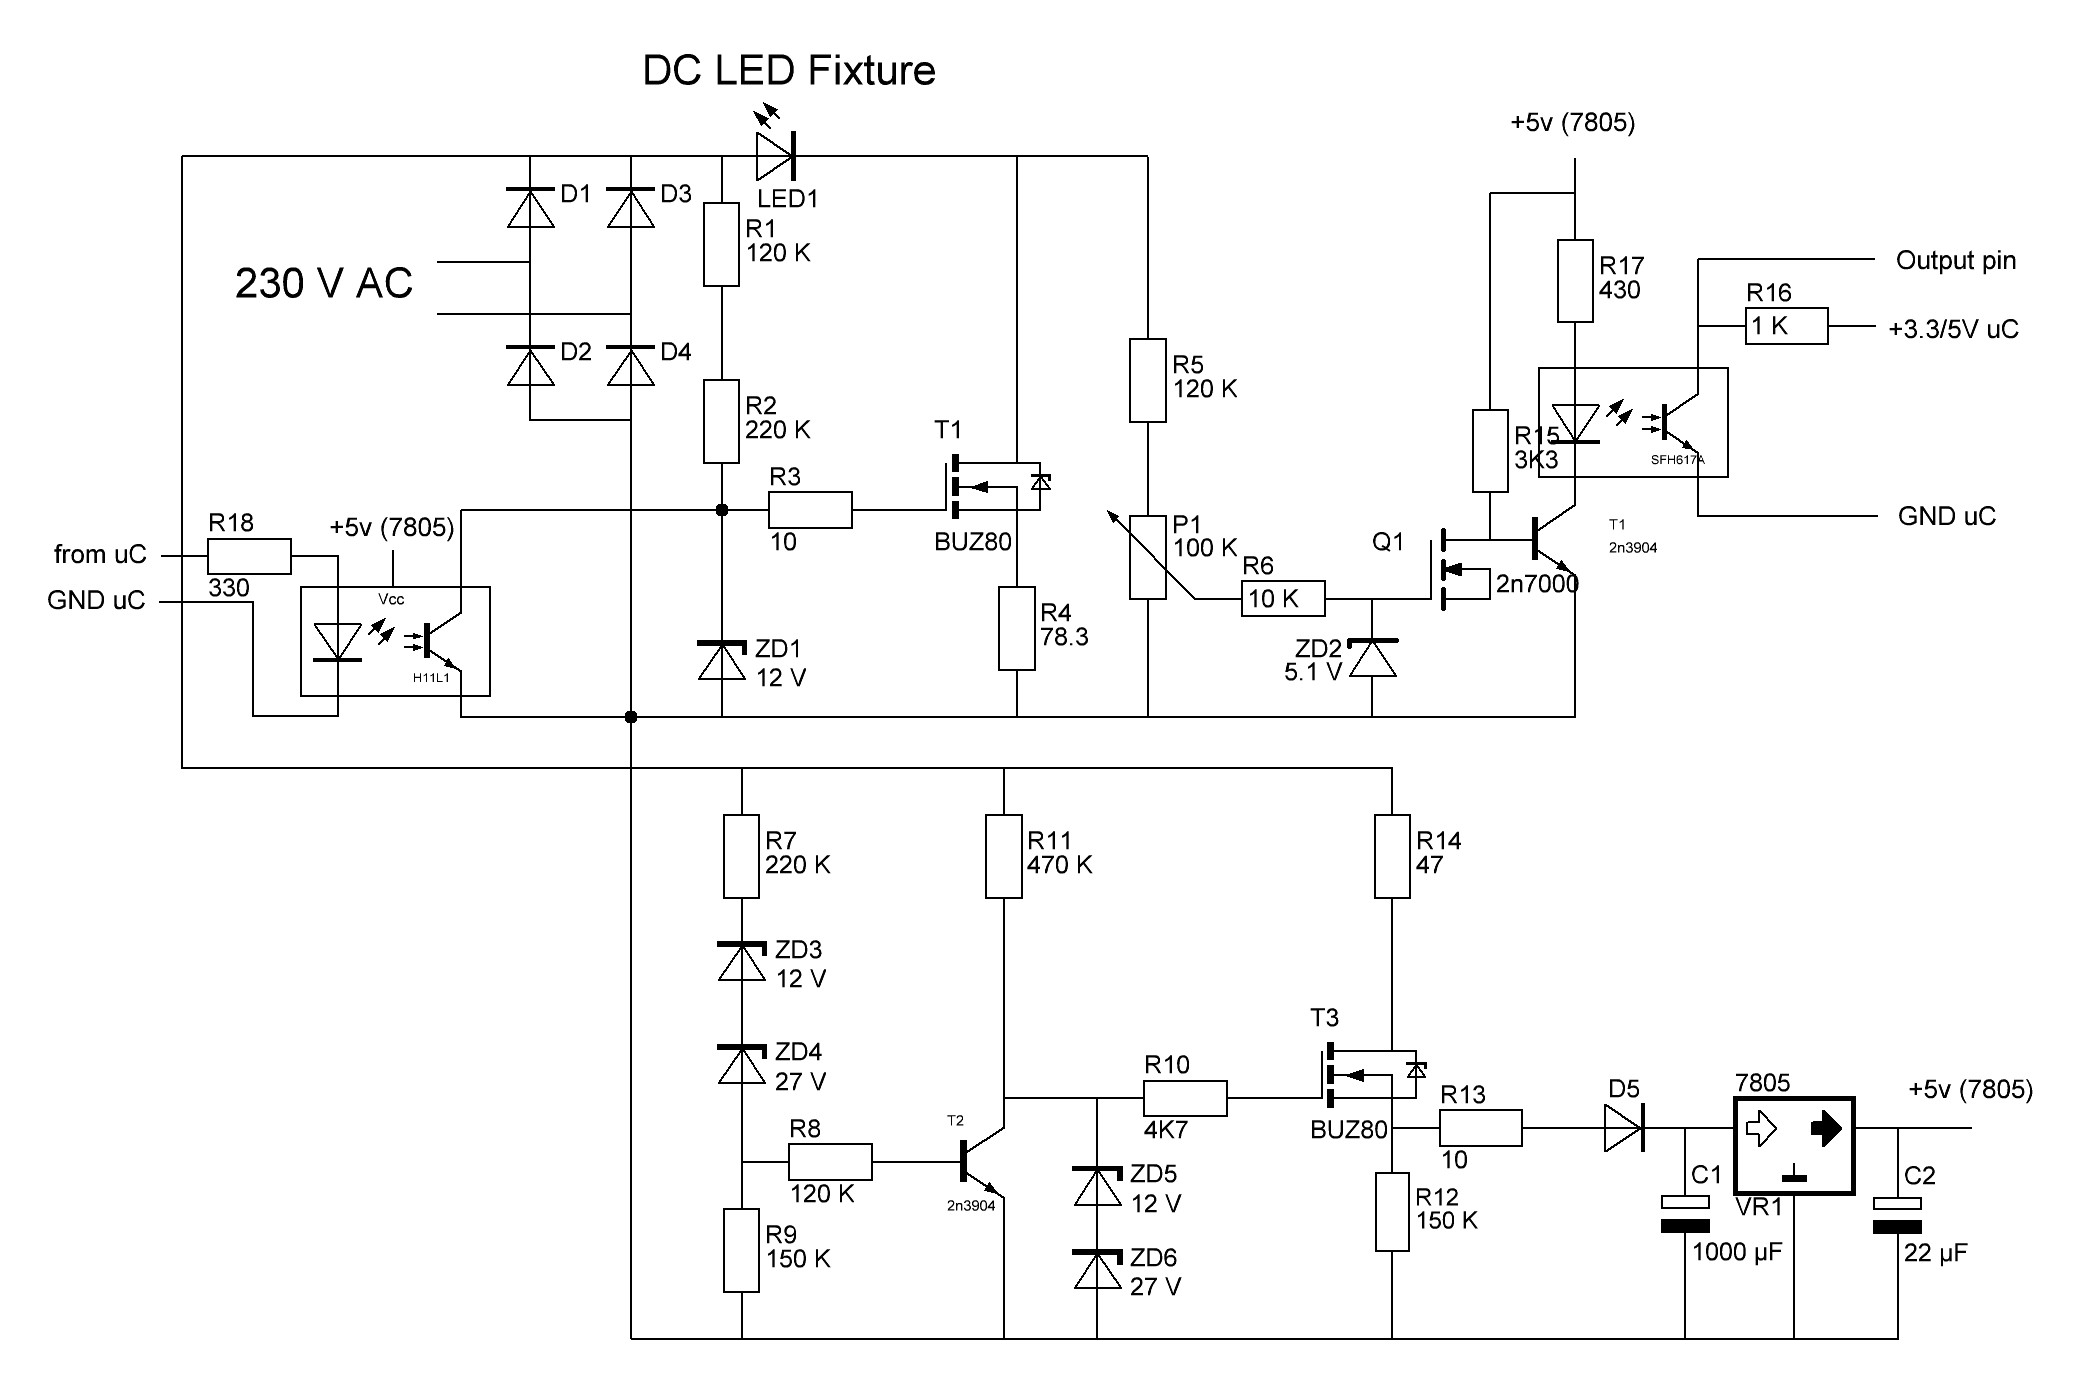
\includegraphics[angle=90,width=\textwidth,height=.9\textheight,keepaspectratio]{chapters/appendix/custom-modulator/custom-modulator-schematic.jpg}
	\caption{Schematic of the LED modulator consisting of a current source with optocoupler, triggering circuit with optocoupler and non-disturbing voltage source.}
	\label{fig:custom-led-modulator-schematic}
\end{figure}


% !TeX root = ../../../thesis.tex

\chapter{Custom Current Sampler Schematic}
\label{app:custom-current-sampler-schematic}

In this chapter, the schematic of the current sampler used to measure the current of the 230 V AC can be found in \autoref{fig:custom-current-sampler-schematic}.
The relevant datasheets for parts used can be found in: \cite{lm7824-vr-datasheet}, \cite{lm7805-vr-datasheet}, \cite{lm336z-ref-voltage-datasheet}, \cite{mcp3204-adc-datasheet}, \cite{iso7241m-spi-isolator-datasheet}, \cite{2n7000-n-fet-datasheet} and \cite{sfh617a-optocoupler-datasheet}.


\begin{figure}[htb]
	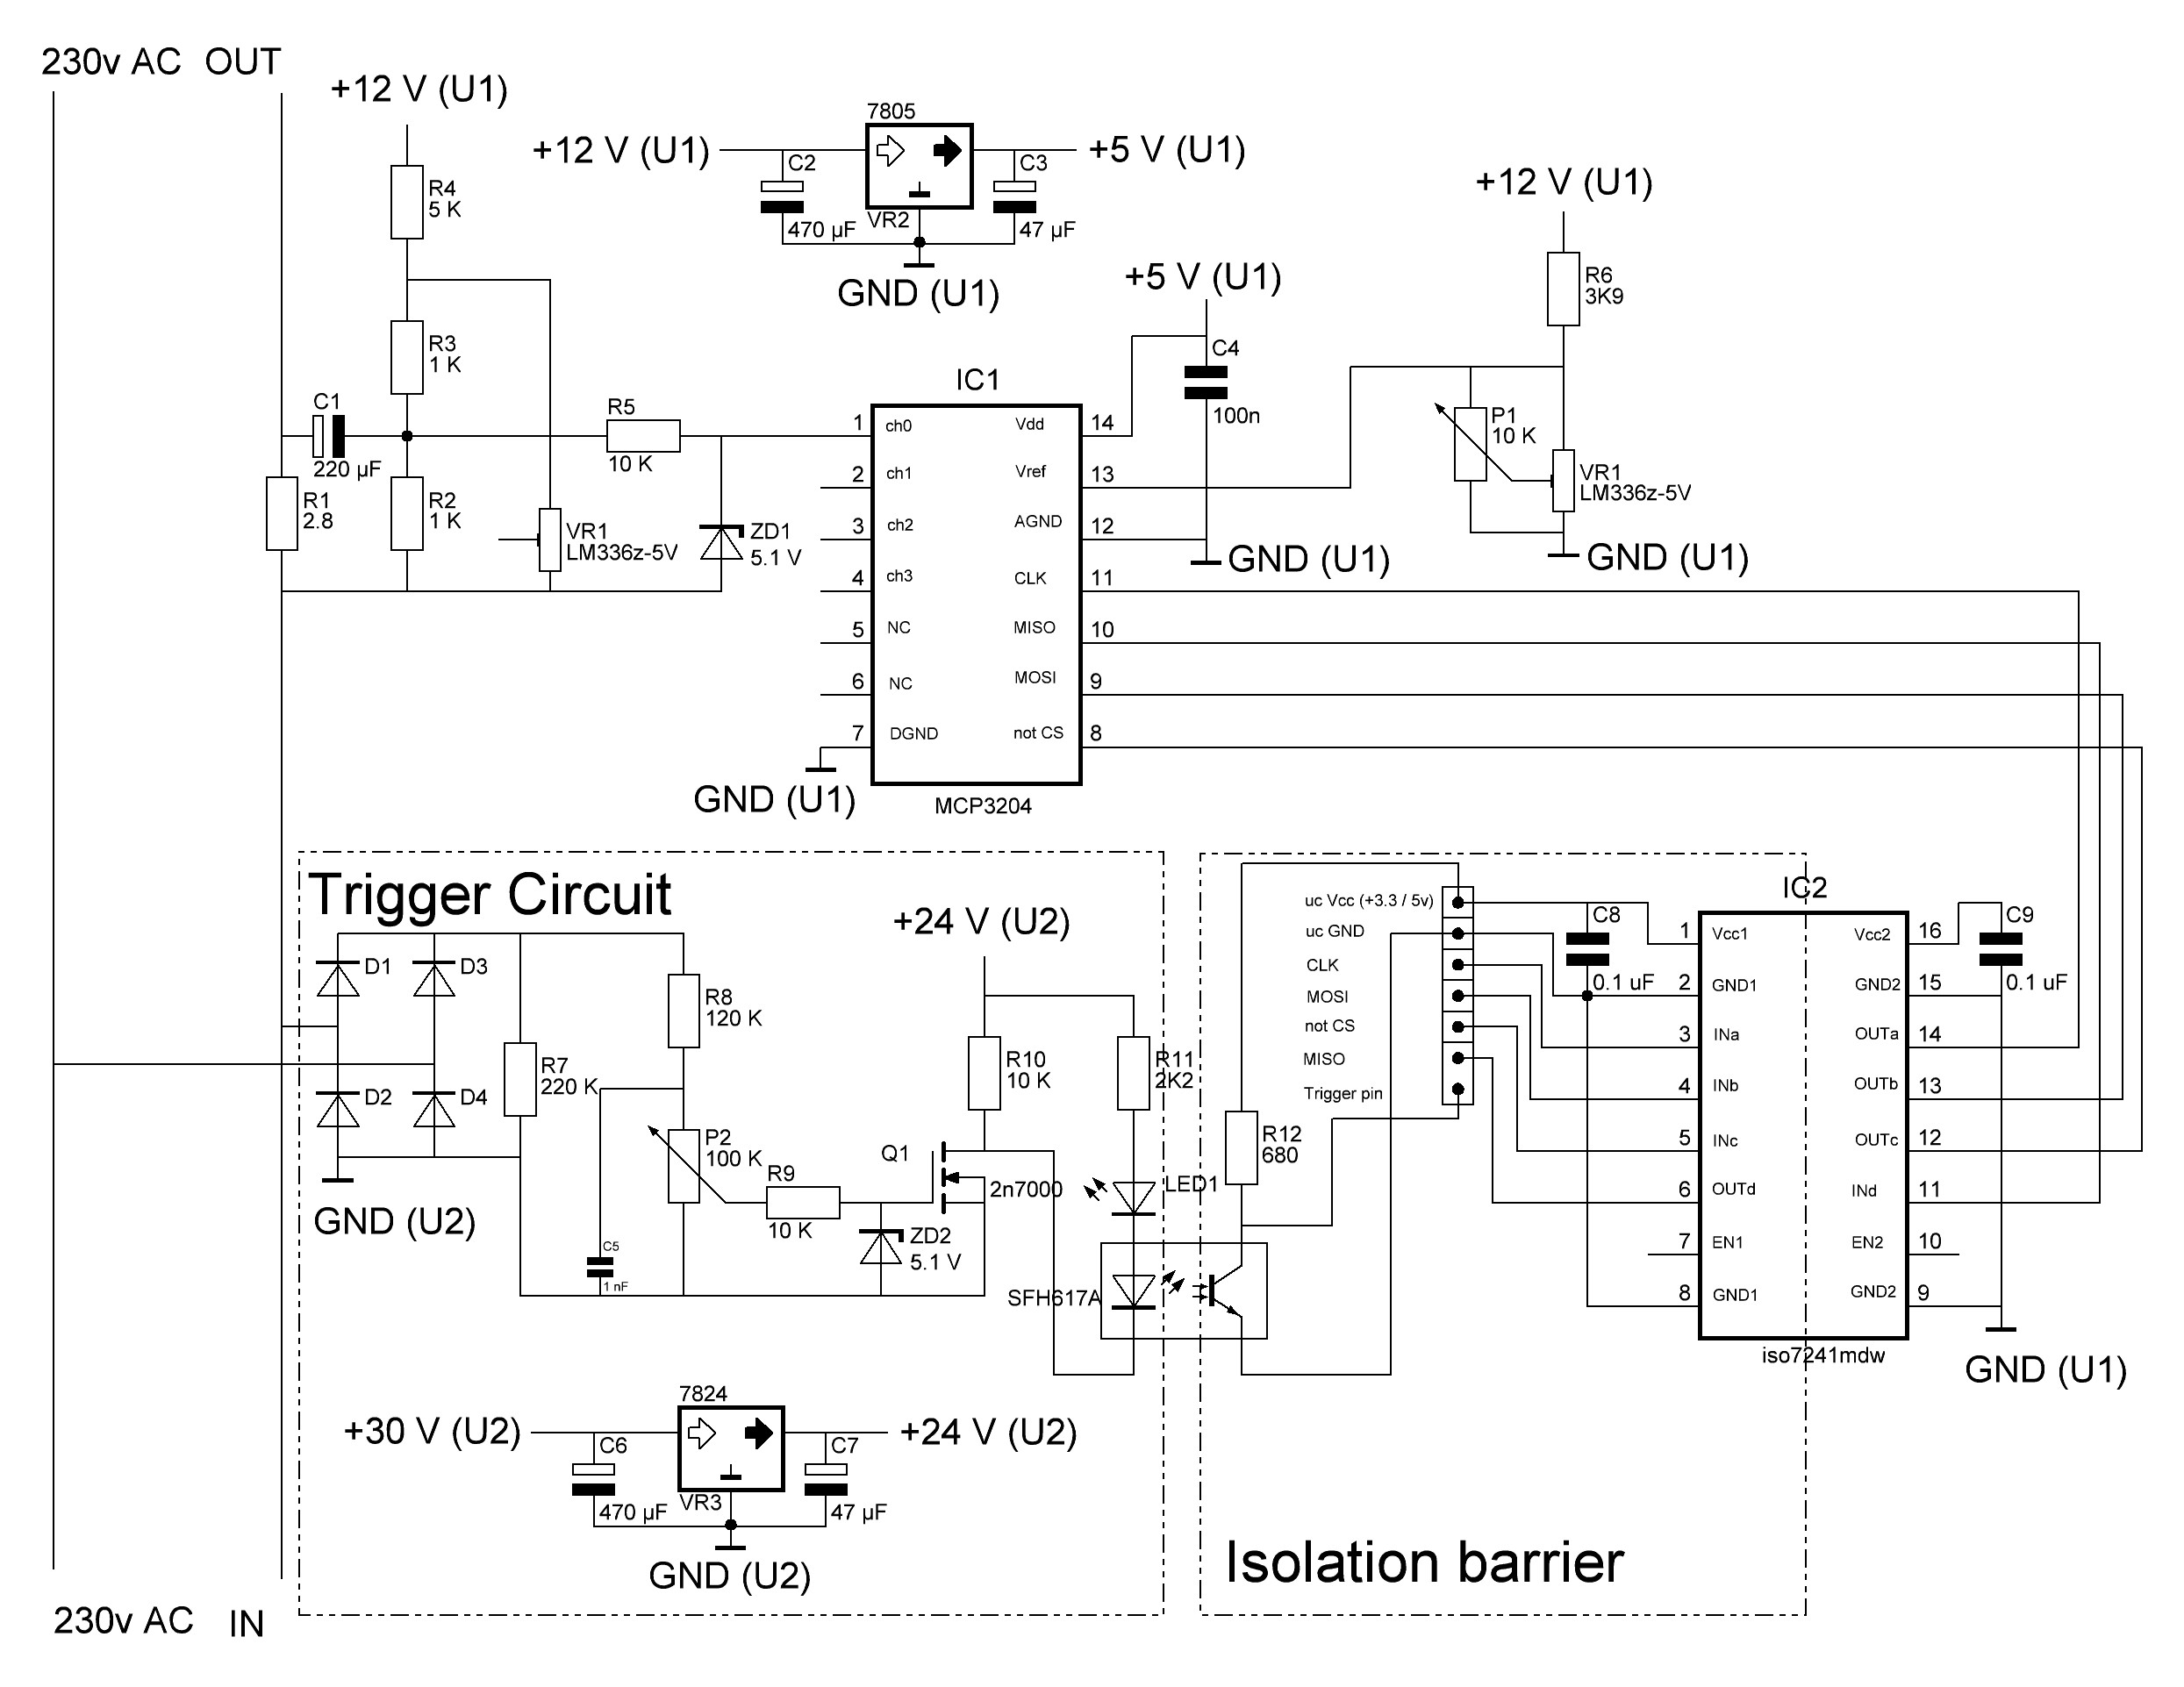
\includegraphics[angle=90,width=\textwidth,height=.9\textheight,keepaspectratio]{chapters/appendix/custom-current-sampler/custom-current-sampler-schematic.jpg}
	\caption{Schematic of the current sampler, with an external ADC which is isolated from the microprocessor and with a triggering circuit.}
	\label{fig:custom-current-sampler-schematic}
\end{figure}



\end{document}

